%%%%%%%%%%%%%%%%%%%%%%%%%%%%%%%%%%%%%%%%%%%%%%%%%%%%
% Document type, global settings, and packages
%%%%%%%%%%%%%%%%%%%%%%%%%%%%%%%%%%%%%%%%%%%%%%%%%%%%

\documentclass[12pt]{report}   %12 point font for Times New Roman
\usepackage{graphicx,caption}  %for images and plots
\usepackage[letterpaper, left=1.5in, right=1in, top=1in, bottom=1in]{geometry}
\usepackage{setspace}  %use this package to set linespacing as desired
\usepackage{times}  %set Times New Roman as the font
\usepackage[explicit]{titlesec}  %title control and formatting
\usepackage[titles]{tocloft}  %table of contents control and formatting
\usepackage[backend=bibtex, sorting=none, bibstyle=ieee]{biblatex}  %reference manager
\usepackage[bookmarks=true, hidelinks]{hyperref}
\usepackage[page]{appendix}  %for appendices
\usepackage{rotating}  %for rotated, landscape images
\usepackage[normalem]{ulem}  %for italicized text
\usepackage{amsmath}
\usepackage{amsfonts}
\usepackage{bm}
\usepackage{bbm}
\usepackage{mathrsfs}
%\usepackage{varioref}
%\usepackage{hyperref}
%\labelformat{algocf}{\textit{alg.}\,(#1)}
%\usepackage{algorithm,algpseudocode}
\usepackage[ruled,vlined]{algorithm2e}
%\usepackage{pythonhighlight}
\usepackage{listings}
\usepackage{booktabs}
\usepackage{subcaption}
%\usepackage[table,xcdraw]{xcolor}
\usepackage{color}
\def\changemargin#1#2{\list{}{\rightmargin#2\leftmargin#1}\item[]}
\let\endchangemargin=\endlist

\definecolor{dkgreen}{rgb}{0,0.6,0}
\definecolor{gray}{rgb}{0.5,0.5,0.5}
\definecolor{lightgray}{rgb}{0.97,0.97,0.97}
\definecolor{mauve}{rgb}{0.58,0,0.82}

\lstnewenvironment{code}[1][]%
{
   \noindent
   \minipage{\linewidth} 
   \lstset{xleftmargin=35pt,
  xrightmargin=35pt,
  backgroundcolor=\color{lightgray},
  language=Python,
  aboveskip=3mm,
  belowskip=3mm,
  showstringspaces=false,
  columns=flexible,
  basicstyle={\small\ttfamily},
  numbers=none,
  numberstyle=\tiny\color{gray},
  keywordstyle=\color{blue},
  commentstyle=\color{dkgreen},
  stringstyle=\color{mauve},
  breaklines=true,
  breakatwhitespace=true,
  tabsize=4,#1
} }
{\endminipage}
%{\endminipage}



% fields
\newcommand{\R}{\mathbb{R}}
\newcommand{\C}{\mathbb{C}}
\newcommand{\Z}{\mathbb{Z}}
\newcommand{\N}{\mathbb{N}}

% complex numbers
\renewcommand{\Re}[1]{\operatorname{Re}\left\{#1\right\}}
\renewcommand{\Im}[1]{\operatorname{Im}\left\{#1\right\}}
\newcommand{\conj}[1]{\mkern 1.5mu\overline{\mkern-1.5mu#1\mkern-1.5mu}\mkern 1.5mu}

% probability and stat
\renewcommand{\P}[1]{\operatorname{P}\left(#1\right)}
\newcommand{\E}{\operatorname{E}}
\newcommand{\var}{\operatorname{var}}

% calculus 
\renewcommand{\d}[1]{d#1}

% constants (written in roman, if wanted)
\newcommand{\e}{e}
\renewcommand{\j}{j}

% linear algebra
% 	vector notation
%\newcommand{\vct}[1]{\boldsymbol{#1}}
\newcommand{\vct}[1]{\bm{#1}}
%   matrices
%\newcommand{\mtx}[1]{\boldsymbol{#1}}
\newcommand{\mtx}[1]{\bm{#1}}
% diagonal
\newcommand{\diag}{\operatorname{diag}}
%   block vector
\newcommand{\bvct}[1]{\mathbf{#1}}
%   block matrix
\newcommand{\bmtx}[1]{\mathbf{#1}}
%	inner products
\newcommand{\<}{\langle}
\renewcommand{\>}{\rangle}
% 	transpose, Hermitian, pseudo-inverse
\renewcommand{\H}{\mathrm{H}}
\newcommand{\T}{\mathrm{T}}
\newcommand{\pinv}{\dagger}
%	fundamental subspaces
\newcommand{\Null}{\operatorname{Null}}
\newcommand{\Range}{\operatorname{Range}}
\newcommand{\Span}{\operatorname{Span}}
%	operators
\newcommand{\trace}{\operatorname{trace}}
\newcommand{\rank}{\operatorname{rank}}
\newcommand{\F}{\mathcal{F}}

% sets and topology
\newcommand{\set}[1]{\mathcal{#1}}
\newcommand{\closure}{\operatorname{cl}}	% closure
\newcommand{\interior}{\operatorname{int}}
\newcommand{\boundary}{\operatorname{bd}}
\newcommand{\diameter}{\operatorname{diam}}

% functional analysis
\newcommand{\domain}{\operatorname{dom}}
\newcommand{\epigraph}{\operatorname{epi}}
\newcommand{\hypograph}{\operatorname{hypo}}
\newcommand{\linop}[1]{\mathscr{#1}}	% general linear operator

% optimization
\renewcommand{\L}{\mathcal{L}}
\DeclareMathOperator*{\minimize}{\text{minimize}}
\DeclareMathOperator*{\maximize}{\text{maximize}}
\newcommand{\indicator}{\mathbbm{1}}
\newcommand{\prox}{\operatorname{prox}}

% Complexity
\newcommand{\bigO}{\mathcal{O}}

% Neural Networks
\newcommand{\pool}{\mtx{P}}


%--------------------------------------------------------------------------


\newcommand{\va}{\vct{a}}
\newcommand{\vb}{\vct{b}}
\newcommand{\vc}{\vct{c}}
\newcommand{\vd}{\vct{d}}
\newcommand{\ve}{\vct{e}}
\newcommand{\vf}{\vct{f}}
\newcommand{\vg}{\vct{g}}
\newcommand{\vh}{\vct{h}}
\newcommand{\vi}{\vct{i}}
\newcommand{\vj}{\vct{j}}
\newcommand{\vk}{\vct{k}}
\newcommand{\vl}{\vct{l}}
\newcommand{\vm}{\vct{m}}
\newcommand{\vn}{\vct{n}}
\newcommand{\vo}{\vct{o}}
\newcommand{\vp}{\vct{p}}
\newcommand{\vq}{\vct{q}}
\newcommand{\vr}{\vct{r}}
\newcommand{\vs}{\vct{s}}
\newcommand{\vt}{\vct{t}}
\newcommand{\vu}{\vct{u}}
\newcommand{\vv}{\vct{v}}
\newcommand{\bvv}{\bvct{v}}
\newcommand{\vw}{\vct{w}}
\newcommand{\vx}{\vct{x}}
\newcommand{\vy}{\vct{y}}
\newcommand{\vz}{\vct{z}}
\newcommand{\bvz}{\bvct{z}}
%
\newcommand{\valpha}{\vct{\alpha}}
\newcommand{\bvalpha}{\bvct{\alpha}}
\newcommand{\vbeta}{\vct{\beta}}
\newcommand{\vepsilon}{\vct{\epsilon}}
\newcommand{\vgamma}{\vct{\gamma}}
\newcommand{\vlambda}{\vct{\lambda}}
\newcommand{\vnu}{\vct{\nu}}
\newcommand{\vmu}{\vct{\mu}}
\newcommand{\bvmu}{\bvct{\mu}}
\newcommand{\vphi}{\vct{\phi}}
\newcommand{\vpsi}{\vct{\psi}}
\newcommand{\vtheta}{\vct{\theta}}
\newcommand{\veta}{\vct{\eta}}
\newcommand{\vomega}{\vct{\omega}}
%
\newcommand{\vzero}{\vct{0}}
\newcommand{\vone}{\vct{1}}

%------------------------------------------------

\newcommand{\mA}{\mtx{A}}
\newcommand{\mB}{\mtx{B}}
\newcommand{\mC}{\mtx{C}}
\newcommand{\mD}{\mtx{D}}
\newcommand{\bmD}{\bmtx{D}}
\newcommand{\mE}{\mtx{E}}
\newcommand{\mF}{\mtx{F}}
\newcommand{\mG}{\mtx{G}}
\newcommand{\mH}{\mtx{H}}
\newcommand{\mJ}{\mtx{J}}
\newcommand{\mK}{\mtx{K}}
\newcommand{\mL}{\mtx{L}}
\newcommand{\mM}{\mtx{M}}
\newcommand{\mN}{\mtx{N}}
\newcommand{\mO}{\mtx{O}}
\newcommand{\mP}{\mtx{P}}
\newcommand{\mQ}{\mtx{Q}}
\newcommand{\mR}{\mtx{R}}
\newcommand{\mS}{\mtx{S}}
\newcommand{\mT}{\mtx{T}}
\newcommand{\mU}{\mtx{U}}
\newcommand{\mV}{\mtx{V}}
\newcommand{\mW}{\mtx{W}}
\newcommand{\mX}{\mtx{X}}
\newcommand{\mY}{\mtx{Y}}
\newcommand{\mZ}{\mtx{Z}}
%
\newcommand{\mDelta}{\mtx{\Delta}}
\newcommand{\mLambda}{\mtx{\Lambda}}
\newcommand{\mPhi}{\mtx{\Phi}}
\newcommand{\mPsi}{\mtx{\Psi}}
\newcommand{\mSigma}{\mtx{\Sigma}}
\newcommand{\mUpsilon}{\mtx{\Upsilon}}
%
\newcommand{\mId}{{\bf I}}
\newcommand{\mEx}{{\bf J}}
\newcommand{\mzero}{{\bf 0}}
\newcommand{\mone}{{\bf 1}}

\newcommand{\mAbar}{\underline{\mtx{A}}}
\newcommand{\mRbar}{\underline{\mtx{R}}}
\newcommand{\vebar}{\underline{\vct{e}}}
\newcommand{\vxbar}{\underline{\vct{x}}}
\newcommand{\vybar}{\underline{\vct{y}}}

%------------------------------------------------

\newcommand{\loF}{\linop{F}}
\newcommand{\loG}{\linop{G}}
\newcommand{\loH}{\linop{H}}

%------------------------------------------------

\newcommand{\setA}{\set{A}}
\newcommand{\setB}{\set{B}}
\newcommand{\setC}{\set{C}}
\newcommand{\setD}{\set{D}}
\newcommand{\setE}{\set{E}}
\newcommand{\setF}{\set{F}}
\newcommand{\setG}{\set{G}}
\newcommand{\setH}{\set{H}}
\newcommand{\setI}{\set{I}}
\newcommand{\setJ}{\set{J}}
\newcommand{\setK}{\set{K}}
\newcommand{\setL}{\set{L}}
\newcommand{\setM}{\set{M}}
\newcommand{\setN}{\set{N}}
\newcommand{\setO}{\set{O}}
\newcommand{\setP}{\set{P}}
\newcommand{\setQ}{\set{Q}}
\newcommand{\setR}{\set{R}}
\newcommand{\setS}{\set{S}}
\newcommand{\setT}{\set{T}}
\newcommand{\setU}{\set{U}}
\newcommand{\setV}{\set{V}}
\newcommand{\setW}{\set{W}}
\newcommand{\setX}{\set{X}}
\newcommand{\setY}{\set{Y}}
\newcommand{\setZ}{\set{Z}}


\newcommand\TODO[1]{}
\newcommand{\np}{\\ \hfill \\}

%%%%%%%%%%%%%%%%%%%%%%%%%%%%%%%%%%%
% Bibliography
%%%%%%%%%%%%%%%%%%%%%%%%%%%%%%%%%%%

%Add your bibliography file here
\bibliography{DissertationLib}

% prevent certain fields in references from printing in bibliography
\AtEveryBibitem{\clearfield{issn}}
\AtEveryBibitem{\clearlist{issn}}

\AtEveryBibitem{\clearfield{language}}
\AtEveryBibitem{\clearlist{language}}

\AtEveryBibitem{\clearfield{doi}}
\AtEveryBibitem{\clearlist{doi}}

\AtEveryBibitem{\clearfield{url}}
\AtEveryBibitem{\clearlist{url}}

\AtEveryBibitem{%
  \ifentrytype{online}
    {}
    {\clearfield{urlyear}\clearfield{urlmonth}\clearfield{urlday}}}

%%%%%%%%%%%%%%%%%%%%%%
% Start of Document
%%%%%%%%%%%%%%%%%%%%%%

\begin{document}
\doublespacing  %set line spacing

%%%%%%%%%%%%%%%%%%%%%%%%%%%%%%%%%%%%%
% Title Page
%%%%%%%%%%%%%%%%%%%%%%%%%%%%%%%%%%%%%

%% Define your thesis title, your name, your school, and your month and year of graduation here

\newcommand{\thesisTitle}{Multi-Layer Dictionary Learning Using Low-Rank Updates}
\newcommand{\yourName}{Lee Richert}
\newcommand{\yourSchool}{Electrical and Computer Engineering}
\newcommand{\yourMonth}{May}
\newcommand{\yourYear}{2022}

%%%%%%%%%%%%%%%%%%%%%%%%%%%%%%%%%%%%%%%%%%%%%%%%%%%%%%%%%
% Do not edit these lines unless you wish to customize
% the template
%%%%%%%%%%%%%%%%%%%%%%%%%%%%%%%%%%%%%%%%%%%%%%%%%%%%%%%%%



\begin{titlepage}
\begin{center}

\begin{singlespacing}

\textbf{\MakeUppercase{\thesisTitle}}\\
\vspace{10\baselineskip}
A Dissertation\\
Presented to\\
The Academic Faculty\\
\vspace{3\baselineskip}
By\\
\vspace{3\baselineskip}
\yourName\\
\vspace{3\baselineskip}
In Partial Fulfillment\\
of the Requirements for the Degree\\
Doctor of Philosophy in the\\
School of \yourSchool\\
\vspace{3\baselineskip}
Georgia Institute of Technology\\
\vspace{\baselineskip}
\yourMonth{} \yourYear{}
\vfill
Copyright \copyright{} \yourName{} 2021 %\yourYear

\end{singlespacing}

\end{center}
\end{titlepage}



\currentpdfbookmark{Title Page}{titlePage}  %add PDF bookmark for this page

%%%%%%%%%%%%%%%%%%%%%%%%%%%%%%%%%%%%%
% Approval Page
%%%%%%%%%%%%%%%%%%%%%%%%%%%%%%%%%%%%%

%% Define your committee members. If you have less than 6, simple delete/comment the unused lines

\newcommand{\committeeMemberOne}{Dr. David V. Anderson}
\newcommand{\committeeMemberOneDepartment}{School of Electrical and Computer Engineering}
\newcommand{\committeeMemberOneAffiliation}{Georgia Institute of Technology}

\newcommand{\committeeMemberTwo}{Dr. Mark A. Davenport}
\newcommand{\committeeMemberTwoDepartment}{School of Electrical and Computer Engineering}
\newcommand{\committeeMemberTwoAffiliation}{Georgia Institute of Technology}

\newcommand{\committeeMemberThree}{Dr. Justin Romberg}
\newcommand{\committeeMemberThreeDepartment}{School of Electrical and Computer Engineering}
\newcommand{\committeeMemberThreeAffiliation}{Georgia Institute of Technology}

%\newcommand{\committeeMemberFour}{Dr. Ashwin Pananjady}
%\newcommand{\committeeMemberFourDepartment}{School of Industrial and Systems Engineering and School of Electrical and Computer Engineering}
%\newcommand{\committeeMemberFourAffiliation}{Georgia Institute of Technology}

%\newcommand{\committeeMemberFive}{Dr. Jacob Abernethy}
%\newcommand{\committeeMemberFiveDepartment}{School of Computer Science}
%\newcommand{\committeeMemberFiveAffiliation}{Georgia Institute of Technology}


\newcommand{\approvalDay}{22}
\newcommand{\approvalMonth}{November}
\newcommand{\approvalYear}{2021}

%%%%%%%%%%%%%%%%%%%%%%%%%%%%%%%%%%%%%%%%%%%%%%%%%%%%%%%%%
% Do not edit these lines unless you wish to customize
% the template
%%%%%%%%%%%%%%%%%%%%%%%%%%%%%%%%%%%%%%%%%%%%%%%%%%%%%%%%%


\begin{titlepage}
\begin{singlespacing}
\begin{center}

\textbf{\MakeUppercase{\thesisTitle}}\\
\vspace{10\baselineskip}

\end{center}
\vfill

%Define minipages, depending on how many authors there are
\ifdefined\committeeMemberFour

Approved by:
\vspace{2\baselineskip}		%adjust the number in front of "\baselineskip" for alignment

\begin{minipage}[b]{0.4\textwidth}
	
	\committeeMemberOne\\
	\committeeMemberOneDepartment\\
	\textit{\committeeMemberOneAffiliation}\\
	
	\committeeMemberTwo\\
	\committeeMemberTwoDepartment\\
	\textit{\committeeMemberTwoAffiliation}\\
	
	\committeeMemberThree\\
	\committeeMemberThreeDepartment\\
	\textit{\committeeMemberThreeAffiliation}\\
	
	\vspace{2\baselineskip}		%adjust the number in front of "\baselineskip" for alignment
	
\end{minipage}
\hspace{0.1\textwidth}
\begin{minipage}[b]{0.4\textwidth}
	
	\committeeMemberFour\\
	\committeeMemberFourDepartment\\
	\textit{\committeeMemberFourAffiliation}\\
	
	\ifdefined\committeeMemberSix
	\committeeMemberFive\\
	\committeeMemberFiveDepartment\\
	\textit{\committeeMemberFiveAffiliation}\\
	
	\committeeMemberSix\\
	\committeeMemberSixDepartment\\
	\textit{\committeeMemberSixAffiliation}\\
	
	Date Approved: \approvalMonth{} \approvalDay, \approvalYear
	\vspace{1\baselineskip}		%adjust the number in front of "\baselineskip" for alignment
	
	\else
	
	\committeeMemberFive\\
	\committeeMemberFiveDepartment\\
	\textit{\committeeMemberFiveAffiliation}\\
		
	Date Approved: \approvalMonth{} \approvalDay, \approvalYear
	\vspace{5\baselineskip}		%adjust the number in front of "\baselineskip" for alignment
	
	\fi
	
\end{minipage}

\else

\hspace{0.6\textwidth}
\begin{minipage}[b]{0.4\textwidth}
	
	Approved by:
	\vspace{2\baselineskip}		%adjust the number in front of "\baselineskip" for alignment
	
	\committeeMemberOne\\
	\committeeMemberOneDepartment\\
	\textit{\committeeMemberOneAffiliation}\\
	
	\committeeMemberTwo\\
	\committeeMemberTwoDepartment\\
	\textit{\committeeMemberTwoAffiliation}\\
	
	\committeeMemberThree\\
	\committeeMemberThreeDepartment\\
	\textit{\committeeMemberThreeAffiliation}\\
	
	\vspace{2\baselineskip}		%adjust the number in front of "\baselineskip" for alignment
	
	Date Approved: \approvalMonth{} \approvalDay, \approvalYear
	\vspace{\baselineskip}		%adjust the number in front of "\baselineskip" for alignment
	
\end{minipage}

\fi





\end{singlespacing}
\end{titlepage}


%%%%%%%%%%%%%%%%%%%%%%%%%%%%%%%%%%%%%
% Epigraph
%%%%%%%%%%%%%%%%%%%%%%%%%%%%%%%%%%%%%

%% Define your quote and author for the epigraph here

\newcommand{\yourQuote}{A great quote to start the thesis}
\newcommand{\yourAuthor}{George P. Burdell}

%%%%%%%%%%%%%%%%%%%%%%%%%%%%%%%%%%%%%%%%%%%%%%%%%%%%%%%%%
% Do not edit these lines unless you wish to customize
% the template
%%%%%%%%%%%%%%%%%%%%%%%%%%%%%%%%%%%%%%%%%%%%%%%%%%%%%%%%%

\begin{titlepage}
\begin{center}

\vspace*{\fill}
\yourQuote\\
\textit{\yourAuthor}
\vspace*{\fill}

\end{center}
\end{titlepage}



%%%%%%%%%%%%%%%%%%%%%%%%%%%%%%%%%%%%%
% Dedication
%%%%%%%%%%%%%%%%%%%%%%%%%%%%%%%%%%%%%

%% Define your dedication statement here

\newcommand{\yourDedication}{A great dedication goes here.}

%%%%%%%%%%%%%%%%%%%%%%%%%%%%%%%%%%%%%%%%%%%%%%%%%%%%%%%%%
% Do not edit these lines unless you wish to customize
% the template
%%%%%%%%%%%%%%%%%%%%%%%%%%%%%%%%%%%%%%%%%%%%%%%%%%%%%%%%%

\begin{titlepage}
\begin{center}

\vspace*{\fill}
\yourDedication\\
\vspace*{\fill}

\end{center}
\end{titlepage}


%%%%%%%%%%%%%%%%%%%%%%%%%%%%%%%%%%%%%
% Acknowledgments
%%%%%%%%%%%%%%%%%%%%%%%%%%%%%%%%%%%%%

\pagenumbering{roman}
\addcontentsline{toc}{chapter}{Acknowledgments}
\setcounter{page}{3} % set the page number appropriately based on the number of intro pages
\clearpage
\begin{centering}
\textbf{ACKNOWLEDGEMENTS}\\
\vspace{\baselineskip}
\end{centering}

I would like to acknowledge and thank my advisor Dr. David Anderson for his guidance and mentorship. I would also like to thank my brother Trip for the many hours of invaluable conversations about software design and development.  
%Insert your dedication text here


\clearpage
%\pagenumbering{gobble}  %remove page number on summary page


\addtocontents{toc}{\cftpagenumbersoff{chapter}} 

\currentpdfbookmark{Acknowledgments}{acknowledgments}
\addtocontents{toc}{\cftpagenumberson{chapter}} 

%%%%%%%%%%%%%%%%%%%%%%%%%%%%%%%%%%%%%
% Table of Contents
%%%%%%%%%%%%%%%%%%%%%%%%%%%%%%%%%%%%%

% Format for Table of Contents
\renewcommand{\cftchapdotsep}{\cftdotsep}  %add dot separators
\renewcommand{\cftchapfont}{\bfseries}  %set title font weight
\renewcommand{\cftchappagefont}{}  %set page number font weight
\renewcommand{\cftchappresnum}{Chapter }
\renewcommand{\cftchapaftersnum}{:}
\renewcommand{\cftchapnumwidth}{5em}
\renewcommand{\cftchapafterpnum}{\vskip\baselineskip} %set correct spacing for entries in single space environment
\renewcommand{\cftsecafterpnum}{\vskip\baselineskip}  %set correct spacing for entries in single space environment
\renewcommand{\cftsubsecafterpnum}{\vskip\baselineskip} %set correct spacing for entries in single space environment
\renewcommand{\cftsubsubsecafterpnum}{\vskip\baselineskip} %set correct spacing for entries in single space environment

%format title font size and position (this also applys to list of figures and list of tables)
\titleformat{\chapter}[display]
{\normalfont\bfseries\filcenter}{\chaptertitlename\ \thechapter}{0pt}{\MakeUppercase{#1}}

\renewcommand\contentsname{Table of Contents}

\begin{singlespace}
\tableofcontents
\end{singlespace}

\currentpdfbookmark{Table of Contents}{TOC}

\clearpage



%%%%%%%%%%%%%%%%%%%%%%%%%%%%%%%%%%%%%
% List of figures and tables
%%%%%%%%%%%%%%%%%%%%%%%%%%%%%%%%%%%%%

\addcontentsline{toc}{chapter}{List of Tables}
\begin{singlespace}
	\setlength\cftbeforetabskip{\baselineskip}  %manually set spacing between entries
	\listoftables
\end{singlespace}

\clearpage

\addcontentsline{toc}{chapter}{List of Figures}
\begin{singlespace}
\setlength\cftbeforefigskip{\baselineskip}  %manually set spacing between entries
\listoffigures
\end{singlespace}

\clearpage

%%%%%%%%%%%%%%%%%%%%%%%%%%%%%%%%%%%%%
% Nomenclature
%%%%%%%%%%%%%%%%%%%%%%%%%%%%%%%%%%%%%
\addcontentsline{toc}{chapter}{Nomenclature}
\clearpage
\begin{centering}
\textbf{NOMENCLATURE}\\
\vspace{\baselineskip}
\end{centering}
\begin{singlespace}
\section*{Acronyms}

\begin{tabular}{cp{0.8\textwidth}}
ADMM & the Alternating Directions Method of Multipliers algorithm\np
ISTA & the Iterative Shrinkage Thresholding Algorithm \np
FISTA & the Fast Iterative Shrinkage Tresholding Algorithm \np
RGB & Describes an image with red, green, and blue channels \np
JPEG & an image compression standard developed by the Joint Photographic Experts Group \np
FFT & the discrete Fourier transform \np
DCT & type-II discrete cosine transform \np
CPU & central processing unit \np
RAM & random-access memory
\end{tabular}

\section*{Integer Constants}
Capital letters that are not bold are used to denote integer constants.\np
\begin{tabular}{cp{0.8\textwidth}}
$M$ & the number of filters\np
$C$ & the number of channels\np
$\hat{K}$ & the number of elements in a single channel of the signal\np
$K$ & the number of elements in a single channel of a filter \np
$\reflectbox{R}$ & a small integer that specifies the rank of the dictionary updates \np
$L$ & the number of layers
\end{tabular}

\section*{Matrices}
Bold capital letters are used to denote matrices.\np
\begin{tabular}{cp{0.8\textwidth}}
$\mD$ & the dictionary. For most of the dissertation, $\mD$ has circulant matrix blocks. \np
%
$\mG$ & another variable used to represent the dictionary. $\mG$ is used when it is necessary to distinguish $2$ different dictionaries, like when dictionary $\mD$ is used to approximate dictionary $\mG$. \np
%
$\mS$ & a collection of signal vectors, either gathering multiple channels or multiple samples. \np
%
$\mX$ & a collection of dictionary coefficient vectors, corresponding to multple signal vectors. \np
%
$\mA$, $\mB$  & the linear operators appearing the the affine constraints for ADMM. $\mA$ and $\mB$ are also used as arbitary matrices when discussing general linear algebra principles. \np
%
$\mU$, $\mV$ & arbitrary matrices used for discussing general linear algebra principles and low-rank updates. \np
%
$\mPhi$ & an arbitrary linear operator \np
%
$\mT$ & a diagonal matrix that has diagonal elements of $1$ for dictionary elements that are not constrained to be zero, and zeros for the other diagonal elements \np
%
$\mW$ & a matrix which converts an image vector from RGB to YUV, downsamples the UV channels, and computes the DCT  of $8 \times 8$ blocks. \np
%
$\mSS$ & part of the dictionary for the product dictionary model \np
%
$\mQ$ & used to denote the matrix $\rho\mId + \hat{\mD}^H\hat{\mD}$ \np
%
$\mXi$ & used to denote the matrix $\rho\mId + \hat{\mD}\hat{\mD}^H$ \np
%
$\mR$ & a rescaling matrix, used to scale a normalized dictionary back to its unnormalized form
\end{tabular}

\section*{Vectors}
Bold, lower-case letters are used to denote vectors.\np
\begin{tabular}{cp{0.8\textwidth}}
$\vx$, $\vy$ & the primal variables for ADMM. \np
%
$\vu$ & the dual variable for ADMM. \np
%
$\vc$ & the constraint vector in ADMM. \np
%
$\vx$, $\vz$ & the coefficients for dictionary model in ADMM algorithm. \np
%
$\vz$ & also used as arbitrary complex vector.\np
%
$\vv$ & another primal variable (grouped with $\vz$) used in chapter $4$. \np
%
$\vgamma$ & the corresponding dual variable. \np
%
$\vx$, $\vz$ & also used as vectors in the FISTA algorithm. \np
%
$\vx$ & also used as an arbitrary vector throughout document.  Context will make clear. \np
%
$\vs$ & the signal. \np
%
$\vb$ & another arbitrary vector. \np
%
$\vu$, $\vv$ & more arbitrary vectors, usually used in pairs. The may collectively specify a rank-$1$ update to a matrix: $\vu\vv^H$. \np
%
$\vf$ & a dictionary filter. \np
%
$\vd$ & a column of $\mD$. \np
%
$\vq$ & the quality-factor dependent vector used in quantization in JPEG compression. \np
%
$\vomega$ & an eigenvector.
\end{tabular}



\section*{Non-Integer Scalars}
Lower-case letters that are not bold are generally used to denote scalars that are not integer constants. $\mathbb{L}$ and $\loss$ are the exceptions.\np
\begin{tabular}{cp{0.8\textwidth}}
$a$, $b$ & arbitrary scalars. \np
%
$\rho$ & a scalar for the ADMM alrogithm that specifies both the weighting of the constraints in the augmented Lagrangian and the stepsize in the dual variable update. \np
%
$\alpha$ & the over-relaxation or under-relaxation factor for ADMM \np
%
$\lambda$ & the factor for the $\operatorname{L}_1$ penalty.  $\lambda$ is also used as the factor for the $\operatorname{L}_2$ penalty on the image gradients for Tikhonov regularization. Context will make clear. \np
%
$\mu$ & the factor for the $\operatorname{L}_2$ penalty for the reconstruction of the signal or coefficients from the previous layer. \np
%
$\mathbb{L}$ & an estimate of the Lipshitz constant, used to determine stepsize in the ISTA and FISTA algorithms. \np
%
$\tau$ & the eigenvalue \np
%
$\eta_{\vu,\vv}$ & used to represent $\vu^H\hat{\mD}\vv$ \np
%
$\eta_{\vu}$ & used to represent $\|\mD^H\vu\|_2^2$ \np
%
$\eta_{\vv}$ & used to represent $\|\vv\|_2^2$ \np
%
$r$, $\omega$ & used to specify momentum stepsize in FISTA and a FISTA-like algorithm. Both always appear with superscripts specifying iteration. \np
%
$\loss$ & loss (as in the loss function)
\end{tabular}

\section*{Functions and Operations}
\begin{tabular}{cp{0.8\textwidth}}
$*$ & Circular convolution \np
%
$a^{*}$ & the complex conjugate of $a$. \np
%
$\vu^H$, $\mU^H$ & the Hermitian transpose of a vector $\vu$ or matrix $\mU$ \np
%
$\L_{\rho}$ & the augmented Lagrangian function \np
%
$\operatorname{S}$ & the shrinkage operator \np
%
$\F$ & applies the Fourier tranform to each channel and/or filter \np
%
$f$ and $g$ & arbitrary convex functions. $f$ may also be used to specify the objective function of a minimization problem. $f$ and $g$ are also used for arbitrary functions that are part of a composite function. Context should make clear. \np
%
$\operatorname{q}(\cdot)$ & quantizes a vector \np
%
$\indicator_{\text{condition}}$ & takes on a value of $0$ when the condition is true and $\infty$ when the condition is false. \np
%
$\arg \min$ & the argument minimum of an expression \np
%
$\nabla_{a} b$ & the gradient of $b$ in respect to $a$ \np
%
$L_1$,$\|\cdot\|_1$ & the $L_1$ norm \np
%
$L_2$,$\|\cdot\|_2$ & the $L_2$ norm \np
%
$\mPhi$ & n arbitrary linear operator (this operator is also listed under matrices, since matrices are linear operators) \np
%
$\mT$ & zeros out all dictionary elements that are constrained to be zero. (This operator is also listed under matrices since matrices are linear operators.) \np
%
$\mW$ & converts from RGB to YUV, downsamples the UV channels, and computes the DCT  of $8 \times 8$ blocks. (This operator also appears under matrices.) \np
%
$\real$ & selects the real component of a complex number, vector, or matrix \np
%
$\imag$ & selects the imaginary component of a complex number, vector, or matrix. (Output is real.)
\end{tabular}
\section*{Superscripts}
\begin{tabular}{cp{0.8\textwidth}}
$a^b$ & An exponent: the $b^{\text{th}}$ power of $a$ \np
%
$a^*$ & the complex conjugate of $a$ \np
%
$\vu^H$, $\mU^H$ & the Hermitian transpose of vector $\vu$ or matrix $\mU$ \np
%
$i^{\text{th}}$ & occuring at position $i$ in a sequence \np
%
$\vgamma^{(t)}$ & the value of vector $\vgamma$ at the $t^{\text{th}}$ iteration \np
%
$\mD^{(n)}$ & the value of dictionary $\mD$ at the $n^{\text{th}}$ dictionary update\np
%
$\nabla_a^{(\vx \rightarrow \vy)} \loss$ & the gradient term of $\loss$ in respect to $a$ that corresponds to the computation of $\vy$ from $\vx$. The gradient of $\loss$ in respect to $a$ is the sum of all the gradient terms.
\end{tabular}

\section*{Subscripts}
\begin{tabular}{cp{0.8\textwidth}}
$m$ & specifies the filter. If there are multiple layers, $[m]$ will be used instead of subscript $m$. \np
%
$n$ & specifies the sample. \np
%
$c$ & specifies the channel. If there are multiple layers $[c]$ will be used instead of subscript $c$. \np
%
$\ell$ & specifies the layer. \np
%
$+$ and $-$ & used to specify the eigenvalues or eigenvectors of a $2 \times 2$ matrix corresponding to the plus or minus in the quadratic formula. \np
%
$\rho$ in $\L_{\rho}$ & specifies the scalar weight of the $L_2$ norm related to the affine constraints, used in the augmented Lagrangian function. \np
%
init in $\mD_{\text{init}}$ & short for initial value, appears in algorithms. \np
%
sc in $\vgamma_{\text{sc}}$ & short for "scaled", and indicates that the variable in the algorithm is a scaled form of the variable. \np
%
$i$ & used for essentially all other subscript indexing.
\end{tabular}

\section*{Indexing Integers}
Lower case letters that are not bold are also used to denote indexing integers.\np
\begin{tabular}{cp{0.8\textwidth}}
$n$ & selects the dictionary update or corresponding signal \np
%
$t$ & selects the iteration \np
%
$m$ & selects the filter \np
%
$c$ & selects the channel \np
%
$\hat{k}$ & specifies the frequency \np

$i$ & used for most other indexing.
\end{tabular}



\end{singlespace}
\clearpage


\addtocontents{toc}{\cftpagenumbersoff{chapter}} 

\currentpdfbookmark{Nomenclature}{nomenclature}
\addtocontents{toc}{\cftpagenumberson{chapter}} 


%%%%%%%%%%%%%%%%%%%%%%%%%%%%%%%%%%%%%%%%%%%%%%%%%%%%%%%%%%%%%%%%%
% This is the Summary (abstract should be separate document)
%%%%%%%%%%%%%%%%%%%%%%%%%%%%%%%%%%%%%%%%%%%%%%%%%%%%%%%%%%%%%%%%%
\addcontentsline{toc}{chapter}{Summary}
\clearpage
\begin{centering}
\textbf{SUMMARY}\\
\vspace{\baselineskip}
\end{centering}



%\pagenumbering{gobble}  %remove page number on summary page


%%%%%%%%%%%%%%%%%%%%%%%%%%%%
%
% Chapters
%
%%%%%%%%%%%%%%%%%%%%%%%%%%%%

%%%%%%%%%%%%%%%%%%%%%%
% formatting
%%%%%%%%%%%%%%%%%%%%%%

% resume page numbering for rest of document
\clearpage
\pagenumbering{arabic}
\setcounter{page}{1} % set the page number appropriately

% Adjust chapter title formatting
\titleformat{\chapter}[display]
{\normalfont\bfseries\filcenter}{\MakeUppercase\chaptertitlename\ \thechapter}{0pt}{\MakeUppercase{#1}}  %spacing between titles
\titlespacing*{\chapter}
  {0pt}{0pt}{30pt}	%controls vertical margins on title
  
% Adjust section title formatting
\titleformat{\section}{\normalfont\bfseries}{\thesection}{1em}{#1}

% Adjust subsection title formatting
\titleformat{\subsection}{\normalfont}{\uline{\thesubsection}}{0em}{\uline{\hspace{1em}#1}}

% Adjust subsubsection title formatting
\titleformat{\subsubsection}{\normalfont\itshape}{\thesubsection}{1em}{#1}

%%%%%%%%%%%%%%%%
% Chapter 1
%%%%%%%%%%%%%%%%
\chapter{Introduction}


\section{Dictionaries and Dictionary Learning}
Dictionary models are powerful and versitile tools, useful in denoising \cite{wohlberg2016convolutional}, classification \cite{kong2012dictionary}, anomaly detection \cite{carroll2017outlier}, super-resolution \cite{polatkan2014bayesian}\cite{gu2015convolutional}, inpainting \cite{papyan2017convolutional}, trajectory-basis non-rigid structure from motion \cite{zhu2013convolutional}\cite{chodosh2020use}, and more. Dictionaries are interpretable, and their models are well-suited for incorporating model assumptions using prior knowledge of the data. In some applications, well-performing dictionaries can be learned from very limited data.

The dictionary model decomposes the signal $\vs$ into the dictionary $\mD$ and coefficients $\vx$.
%
\begin{equation}
\vs \approx \mD\vx
\end{equation}
%
When the dictionary is known, solving for $\vx$ using $\mD$ and $\vs$ is a pursuit algorithm. When the dictionary is unknown, learning the dictionary from $\vs$ is called dictionary learning. In this dissertation, I present a novel dictionary learning algorithm specifically for convolutional dictionaries.

\subsection{Convolutional Dictionaries}
\begin{figure}
	
\includegraphics[width=\textwidth]{figures/convolutionalDictionary.png}
	\caption{This is a $1$-dimensional dictionary with convolutional structure. The columns of the dictionary are shifted versions of the dictionary filters.}
	\label{Figure: Convolutional Dictionary}
\end{figure}
The convolutional dictionary model is a dictionary model which imposes a convolutional structure on the dictionary. This structure is shown in Figure \ref{Figure: Convolutional Dictionary}. Note that while the example uses $1$-dimensional convolution, it is straightforward to extend to multi-dimensional convolution through vectorization. The convolutional dictionary model equation can be notated as signals convolved with filters:
%
\begin{equation}
\vs \approx \sum_i \vf_i * \vx_i
\end{equation}
%
where $\vf_i$ is the $i$th filter of the dictionary, $\vx_i$ is the coefficients for the $i$th filter, and $*$ indicates convolution. This structure is useful for signals where shift-invariance is a desirable characteristic and/or when dealing with variable-length data. Convolutional approaches often outperform patch-based methods. For the rest of this dissertation, I will notate $\sum_i \vf_i * \vx_i$ as $\mD\vx$. The matrix $\mD$ consists of $M$ Toeplitz blocks $\mD_{m}$, each block corresponding to a particular filter $m$ of the $M$ dictionary filters.

\section{Multi-Layer Dictionaries}
A multi-layer dictionary treats the coefficients as the signal of a subsequent dictionary model. That is,
\begin{equation}
\begin{split}
\vs \approx & \mD_1\vx_1
\\
\vx_1 \approx & \mD_2\vx_2
\\
\vdots & 
\\
\vx_{L - 1} \approx & \mD_L\vx_L
\end{split}
\end{equation}
where $L$ is the number of layers. Pursuit for a multi-layer dictionary model seeks to find the coefficients for all layers $\vx_1,\vx_2,\hdots,\vx_L$. Multi-layer dictionary models have been used in applications such as feature extraction for classification \cite{chen2013deep}\cite{zeiler2010deconvolutional}\cite{pu2014bayesian} and trajectory-basis non-rigid structure from motion \cite{chodosh2020use}. Dictionary models can often be easily extended to allow the researcher or practitioner to inject prior knowledge into the model architecture through the use of convex constraints or known projection operator $\mPhi$. For convolutional dictionaries, the projection operator $\mPhi$ need not have convolutional structure.
%
\begin{equation}
\begin{split}
\vs \approx \mPhi\mD\vx
\\
\operatorname{f}_i(\vx) \leq b_i \text{ } \forall i
\end{split}
\end{equation}
%
In the context of multi-layer dictionary models, these types of dictionary model modifications have been shown to be useful for applications such as interpolation of LIDAR measurements using RGB imagery \cite{murdock2018deep}\cite{chodosh2018deep} and compression-artifact removal \cite{chodosh2020use}.

Some researchers have noted that convolutional neural networks resemble multi-layer dictionaries \cite{papyan2017convolutional}: thresholding is a type of pursuit algorithm, and rectified linear unit activations perform the same operation. A convolutional neural network is a composite function of convolutionals, pooling functions, and activation functions. Over the last decade, convolutional neural networks have reached state-of-the-art performance on a wide variety of tasks. In a way, multi-layer dictionary models can be thought of as a blend of dictionary models and convolutional neural networks, since multi-layer dictionary models mimic the layered structure of convolutional neural networks, while maintaining the interpretability of dictionary models.


\section{Organization of Dissertation}
In chaper $2$, I derive a novel dictionary learning method for multi-channel signals. In chapter $3$, I show how that approach can be adapted to multi-layer dictionary models.  Finally, in chapter $4$, I apply the multi-layer dictionary approach to JPEG compression artifact removal. Chapter $5$ features some practical considerations when implementing these algorithms.

% This is a figure
%\begin{figure}
%	\includegraphics[width=\textwidth]{figures/exampleFigure.png}
%	\caption{This is an example Figure.}
%	\label{Figure in Chapter 1}
%\end{figure}


% This is a table

%\begin{table}
%\caption{This is an example Table.}
%\begin{center}
%\begin{tabular}{ccc}
%x & f(x) & g(x) \\
%\hline
%1 & 6 & 4  \\
%2 & 6 & 3  \\
%3 & 6 & 2  \\
%4 & 6 & 2  \\
%\label{Table in Chapter 1}
%\end{tabular}
%\end{center}
%\end{table}



%%%%%%%%%%%%%%%%
% Chapter 2
%%%%%%%%%%%%%%%%

\chapter{Learning Dictionaries for Multi-Channel Signals}

\section{Introduction}
Much of the literature on using convolutional dictionaries is tailored to applications with signals that only have a small number of channels (like RGB or grayscale imagery). Many of the methods designed with a small number of channels in mind do not transfer well to applications like hyperspectral imagery \cite{PURR1947} with signal measurements containing a large number of channels.

Signal measurements are not the only way to end up with a large number of channels. In a multi-layer dictionary model, the coefficients corresponding to a dictionary from one layer become the signal for the subsequent layer.  The number of channels for this signal is the number of dictionary filters from the previous layer, so if the number of filters in a layer is large, the number of channels for the subsequent layer will also be large.

This chapter presents a novel method to learn convolutional dictionaries for multi-channel signals. 
\section{Dictionary Types}
There are many ways to construct a convolutional sparse representation of a multi-channel signal. One way models can differ is if and how signal channels share dictionaries and coefficients.

For example, models with single-channel dictionaries represent the channels in the coefficients:\footnote{In this case, both $\mX$ and $\mS$ still refer to a single sample. They are capitalized because they are matrices.}
%
\begin{equation}
\mS \approx \mD\mX
\end{equation}
\begin{equation}
\mS = \begin{bmatrix} \vs_1 & \hdots & \vs_C \end{bmatrix}
\end{equation}
\begin{equation}
\mD = \begin{bmatrix} \mD_1 & \hdots & \mD_M \end{bmatrix}
\end{equation}
\begin{equation}
\mX = \begin{bmatrix} \vx_{1,1} & \hdots & \vx_{1,C} \\ \vdots & \ddots & \vdots \\ \vx_{M,1} & \hdots & \vx_{M,C} \end{bmatrix}
\end{equation}
%
where $\vs_c \in \R^{\hat{K}}$, $\mD_m \in \R^{\hat{K} \times \hat{K}}$, and $\vx_{m,c} \in \R^{\hat{K}}$, using $\hat{K}$ as the number of elements in a single channel of the signal.

Alternatively, each signal channel could be given its own dictionary model.
%
\begin{equation}
\vs_c \approx \mD_c\vx_c
\end{equation}
%
where $\vs_c \in \R^{\hat{K}}$, $\mD_c \in \R^{\hat{K} \times M\hat{K}}$, and $\vx_{c} \in \R^{M\hat{K}}$.

In both the above-mentioned cases, the models use multi-channel coefficients. For multi-layer models, this poses a problem: with each subsequent layer, the number of coefficients grows by a factor of the number of filters. Thus, the number of coefficients increases exponentially in respect to the number of layers.

This exponential growth could be dampened (though not eliminated) through the use of product dictionaries \cite{garcia2018multichannel}. In product dictionary models, correlations between channels are captured in a separate matrix $\mSS$.
%
\begin{equation}
\mS \approx \mD\mX\mSS
\end{equation}
\begin{equation}
\mS = \begin{bmatrix} \vs_1 & \hdots & \vs_C \end{bmatrix}
\end{equation}
\begin{equation}
\mD = \begin{bmatrix} \mD_1 & \hdots & \mD_M \end{bmatrix}
\end{equation}
\begin{equation}
\mX = \begin{bmatrix} \vx_{1,1} & \hdots & \vx_{1,B} \\ \vdots & \ddots & \vdots \\ \vx_{M,1} & \hdots & \vx_{M,B} \end{bmatrix}
\end{equation}
%
where $\vs_c \in \R^{\hat{K}}$, $\mD_m \in \R^{\hat{K} \times \hat{K}}$, $\vx_{m,b} \in \R^{\hat{K}}$, and $\mSS \in \R^{B \times C}$. Pursuit algorithms for product dictionaries still seek to estimate $\mX$ for fixed $\mS$, $\mD$, and $\mSS$. For dictionary learning, $\mSS$ is updated with $\mD$.

For this work, I will instead focus on multi-channel dictionaries with shared coefficients.
%
\begin{equation}
\vs \approx \mD\vx
\end{equation}
\begin{equation}
\vs = \begin{bmatrix} \vs_1 \\ \hdots \\ \vs_C \end{bmatrix}
\end{equation}
\begin{equation}
\mD = \begin{bmatrix} \mD_{1,1} & \hdots & \mD_{1,M}  \\ \vdots & \ddots & \vdots \\ \mD_{C,1} & \hdots & \mD_{C,M} \end{bmatrix}
\end{equation}
\begin{equation}
\vx = \begin{bmatrix} \vx_1 \\ \vdots \\ \vx_M \end{bmatrix}
\end{equation}
where $\vs_c \in \R^{\hat{K}}$, $\mD_{c,m} \in \R^{\hat{K} \times \hat{K}}$, and $\vx_{m} \in \R^{\hat{K}}$, again using $\hat{K}$ to represent the number of elements in one channel of the signal.
%
When extended to multi-layer dictionaries, this structure closely aligns with that of convolutional neural networks,  and the number of channels for a subsequent dictionary is the number of filters for the dictionary from the previous layer. The number of coefficients does not grow exponentially with the number of layers, but the number of channels can be large.



\section{Pursuit and Sparse Coding}
\label{section:sparse coding}
The dictionary model decomposes the signal $\vs_n$ into a dictionary $\mD$ (which generalizes to other signals) and the coefficients $\vx_n$ (which are specific to the signal $\vs_n$):
%
\begin{equation}
\vs_n \approx \mD\vx_n
\end{equation}
%
(Here the subscript $n$ specifies a particular signal and its corresponding coefficients.) A pursuit algorithm finds the coefficients $\vx_n$ corresponding to a particular signal $\vs_n$ for known dictionary $\mD$. If the number of dictionary atoms (columns) is larger than the dimension of the signal, then the number of unknowns is larger than the number of equations, and many solutions for $\vx_n$ represent $\vs_n$ equally well (at least in an $\operatorname{L}_2$ sense). Researchers and practitioners commonly either impose a sparsity constraint on the coefficients or add a coefficient $\operatorname{L}_1$ penalty to the objective function, which removes this ambiguity from the problem construction. When such a penalty or constraint is used, pursuit is sometimes called sparse coding. With the added coefficient $\operatorname{L}_1$ penalty, the pursuit optimization problem looks like this:
%
\begin{equation}\label{equation:sparse coding}
\vx_n = \arg\min_{\vx} \frac{1}{2}\|\vs_n - \mD\vx\|_2^2 + \lambda \|\vx\|_1
\end{equation}
%
where $\lambda$ is a nonnegative hyperparameter controlling how much the $\operatorname{L}_1$ norm of the coefficients is penalized. Researchers have proposed many ways to solve this problem. If the dictionary is convolutional and the number of channels is low, a standard approach is to use the Alternating Direction Method of Multipliers (ADMM) algorithm.

\section{ADMM}
\label{section:ADMM}
ADMM is a convex-optimization algorithm used to solve the optimization problem:
\begin{equation} \label{equation:ADMM}
\begin{aligned}
\minimize_{\vx,\vy} & f(\vx) + g(\vy) \\
\text{subject to } & \mA\vx + \mB\vy + \vc = \vzero 
\end{aligned}
\end{equation}
%
where $f$ and $g$ are convex functions \cite{boyd2011distributed}. (I will address how to put the sparse coding problem in this form in the next section.)

The ADMM algorithm makes use of the augmented Lagrangian, a particular expression that has a saddle point at the solution to the constrained optimization problem:
%
\begin{equation}
\L_{\rho}(\vx,\vy,\vu) = f(\vx) + g(\vy) + \vu^H(\mA\vx + \mB\vy + \vc) + \frac{\rho}{2}\|\mA\vx + \mB\vy + \vc\|_2^2
\end{equation}
%
where $\rho$ is a hyperparameter greater than zero and $\vu$ is the dual variable for the constraints.

At the saddle-point solution, the augmented Lagrangian is at a minimum in respect to $\vx$ and $\vy$, but at a maximum in respect to $\vu$.

The ADMM algorithm is an iterative search for the saddle point of the augmented Lagrangian. Each iteration consists of a primal update for $\vx$, a primal update for $\vy$, and a dual update for $\vu$:
%
\begin{equation}
\vx^{(t + 1)} = \arg\min_{\vx} \L_{\rho}(\vx,\vy^{(t)},\vu^{(t)})
\end{equation}
%
\begin{equation}
\vy^{(t + 1)} = \arg\min_{\vy} \L_{\rho}(\vx^{(t + 1)},\vy,\vu^{(t)})
\end{equation}
%
\begin{equation} \label{equation:general dual update}
\vu^{(t + 1)} = \vu^{(t)} + \rho(\mA\vx^{(t + 1)} + \mB\vy^{(t + 1)} + \vc)
\end{equation}
%
\begin{algorithm}[H] \label{algorithm:ADMM}
\SetAlgoLined
%\KwResult{Write here the result }
 %initialization:\\
   $\vy = $ initial guess \\
   $\vu = \vzero$ \\
 \While{Not Converged}{
  $\vx = \arg \min_{\vx}  \L_{\rho}(\vx,\vy,\vu)$ \\
  $\vy = \arg \min_{\vy} \L_{\rho}(\vx,\vy,\vu)$ \\
  $\vu = \vu + \rho(\mA\vx + \mB\vy + \vc)$
 }
 \caption{ADMM}
\end{algorithm}

The primal updates serve to move towards the minimum of the augmented Lagrangian in respect to $\vx$ and $\vy$ with $\vu$ fixed, and the dual update fixes $\vx$ and $\vy$, and performs gradient ascent on $\vu$ with stepsize $\rho$. Under very mild assumptions, this process converges to a saddle point of the augmented Lagrangian, which matches a solution to the constrained optimization problem.\footnote{Neither the saddle point nor the corresponding solution to the constrained optimization problem are guaranteed to be unique, however.} The ADMM algorithm is shown in Algorithm \ref{algorithm:ADMM}.

There are two common variations of the ADMM algorithm that this dissertation will make use of.  The first is the scaled form, which comes from completing the square for the augmented lagrangian function:
%
\begin{equation}
\L_{\rho}(\vx,\vy,\vu) = f(\vx) + g(\vy) + \frac{\rho}{2}\|\mA\vx + \mB\vy + \vc + \frac{\vu}{\rho}\|_2^2 - \frac{\rho}{2}\|\frac{\vu}{\rho}\|_2^2
\end{equation}
%
The term $-\frac{\rho}{2}\|\frac{\vu}{\rho}\|_2^2$ can be ignored for the primal updates because it has no dependence on the primal variables. It is sometimes more convenient to keep track of $\vu_{\text{sc}} = \frac{\vu}{\rho}$ instead of $\vu$, since that is the form that appears in the augmented Lagrangian after completing the square. The dual update for the scaled form is easily derived from equation \ref{equation:general dual update}.
%
\begin{equation}
\frac{\vu^{(t + 1)}}{\rho} = \frac{\vu^{(t)}}{\rho} + \mA\vx^{(t + 1)} + \mB\vy^{(t + 1)} + \vc
\end{equation}
%
This form is known as scaled ADMM.

Another common variation of ADMM updates the dual variable more frequently \cite{eckstein1994parallel}.
\begin{equation}
\vx^{(t + 1)} = \arg\min_{\vx} \L_{\rho}(\vx,\vy^{(t)},\vu^{(t)})
\end{equation}
%
\begin{equation}
\vu^{(t + \frac{1}{2})} = \vu^{(t)} + (\alpha - 1)\rho(\mA\vx^{(t + 1)} + \mB\vy^{(t)} + \vc)
\end{equation}
%
\begin{equation}
\vy^{(t + 1)} = \arg\min_{\vy} \L_{\rho}(\vx^{(t + 1)},\vy,\vu^{(t + \frac{1}{2})})
\end{equation}
%
\begin{equation}
\vu^{(t + 1)} = \vu^{(t + \frac{1}{2})} + \rho(\mA\vx^{(t + 1)} + \mB\vy^{(t + 1)} + \vc)
\end{equation}
%
When $\alpha > 1$, this is known as over-relaxation, and if $\alpha < 1$, this is known as under-relaxation.\footnote{I have elected to notate over/under relaxation differently than standard notation, but the $\alpha$ is the same, and the notations are mathematically equivalent. The standard notation does not use the first dual update, and instead includes another variable $\vh^{(t + 1)} = \mA\vx^{(t + 1)} - (1 - \alpha)(\mA\vx^{(t + 1)} + \mB\vy^{(t)} + \vc)$ and substitutes $\vh^{(t + 1)}$ for $\mA\vx^{(t + 1)}$ in the dual-update equation and the second primal-update equation. While more familiar to readers who have dealt with ADMM before, this standard notation complicates ADMM with an extra variable and obscures how the dual update and second primal update relate to the augmented Lagrangian.} $\alpha$ is always chozen to be greater than zero. In some applications, researchers have found using over-relaxation converges faster than without over-relaxation \cite{eckstein1994parallel}, but optimal choice of $\alpha$ is problem-dependent \cite{nishihara2015general}. Scaled ADMM with over-relaxation is shown in Algorithm \ref{algorithm:Scaled ADMM with Relaxation}.

\begin{algorithm}[H] \label{algorithm:Scaled ADMM with Relaxation}
\SetAlgoLined
%\KwResult{Write here the result }
 %initialization:\\
   $\alpha \in (0,2]$ \\
   $\vy = $ initial guess \\
   $\vu_{\text{sc}} = \vzero$ \\
 \While{Not Converged}{
  $\vx = \arg \min_{\vx}  \L_{\rho}(\vx,\vy,\rho\vu_{\text{sc}})$ \\
  $\vu_{\text{sc}} = \vu_{\text{sc}} + (\alpha - 1)(\mA\vx + \mB\vy + \vc)$ \\
  $\vy = \arg \min_{\vy} \L_{\rho}(\vx,\vy,\rho\vu_{\text{sc}})$ \\
  $\vu_{\text{sc}} = \vu_{\text{sc}} + \mA\vx + \mB\vy + \vc$
 }
 \caption{Scaled ADMM With Over or Under-Relaxation}
\end{algorithm}


\section{Applying ADMM to the Sparse Coding Problem}
\label{section:Applying ADMM}
Recall from section \ref{section:sparse coding}, equation \ref{equation:sparse coding} for sparse coding.
%
\begin{equation}
\vx_i = \arg\min_{\vx} \frac{1}{2}\|\vs_i - \mD\vx\|_2^2 + \lambda \|\vx\|_1
\end{equation}
%
This can be rewritten to match the ADMM form from equation \ref{equation:ADMM}:
\begin{equation} \label{equation:SC Opt Prob}
\begin{aligned}
\minimize_{\vx,\vy} & \frac{1}{2} \|\vs_i - \mD\vx\|_2^2 + \lambda\|\vy\|_1 \\
         \text{subject to } & \vy - \vx = \vzero
\end{aligned}
\end{equation}
%
Using his form, the ADMM algorithm can be used to solve the sparse coding problem, as shown in Algorithm \ref{algorithm:ADMM for Sparse Coding}. Given sufficient iterations, $\vx$ and $\vy$ will both be close to the optimal, but they may not be equal. Either can be used as an approximate solution to the sparse coding problem.

Computing the augmented Lagrangian of the convex optimization problem in expression \ref{equation:SC Opt Prob} yields the following equation:
%
\begin{equation}
\L_{\rho}(\vx,\vy,\vu) = \frac{1}{2} \|\vs_i - \mD\vx\|_2^2 + \lambda\|\vy\|_1 + \frac{\rho}{2}\|\vy - \vx + \frac{\vu}{\rho}\|_2^2 - \frac{1}{2\rho}\|\vu\|_2^2
\end{equation}
%
Starting with the $\vx$-update:
\begin{equation}
\vx^{(t + 1)} = \arg\min_{\vx} \L_{\rho}(\vx,\vy^{(t)},\vu^{(t)})
\end{equation}
%
Since the desired result is the minimizer, setting the gradient to zero and solving for $\vx$ will produce the solution.
%
\begin{equation}
\nabla_{\vx^{(t + 1)}} \L_{\rho}(\vx^{(t + 1)},\vy{(t)},\vu{(t)}) = \vzero
\end{equation}
%
\begin{equation}
\vzero = \mD^T\mD\vx^{(t + 1)} - \mD^T\vs_i + \rho\vx^{(t + 1)} - \rho\left(\vy^{(t)} + \frac{\vu^{(t)}}{\rho}\right)
\end{equation}
%
\begin{equation}
(\rho\mId + \mD^T\mD)\vx^{(t + 1)} = \mD^T\vs_i + \rho\left(\vy^{(t)} + \frac{\vu^{(t)}}{\rho}\right)
\end{equation}
%
\begin{equation}
\vx^{(t + 1)} = (\rho\mId + \mD^T\mD)^{-1}\left(\mD^T\vs_i + \rho\left(\vy^{(t)} + \frac{\vu^{(t)}}{\rho}\right)\right)
\end{equation}
%
In subsection \ref{subsection:SC xupdate}, there is a discussion of the implications of this update equation, how to compute it for cases in which the signal has a low number of channels, and the challenges it poses for signals with many channels.

If using over-relaxation\footnote{or under-relaxation}, there is a dual update:
\begin{equation}
\frac{\vu^{(t + \frac{1}{2})}}{\rho} = \frac{\vu^{(t)}}{\rho} + (\alpha - 1)(\vy^{(t)} - \vx^{(t + 1)})
\end{equation}
%
Moving on to the $\vy$-update:
\begin{equation}
\vy^{(t + 1)} = \arg\min_{\vy} \operatorname{L}_{\rho}(\vx^{(t + 1)},\vy,\vu^{(t + \frac{1}{2})})
\end{equation}
%
Excluding the terms that don't include $\vy$ yields
\begin{equation}
\vy^{(t + 1)} = \arg\min_{\vy} \lambda\|\vy\|_1 + \frac{\rho}{2}\|\vy - \vx^{(t + 1)} + \frac{\vu^{(t + \frac{1}{2})}}{\rho}\|_2^2
\end{equation}
%
This is a well-known problem, whose solution is
\begin{equation}
\vy^{(t + 1)} = \operatorname{S}_{\frac{\lambda}{\rho}}(\vx^{(t + 1)} - \frac{\vu^{(t + \frac{1}{2})}}{\rho})
\end{equation}
where $\operatorname{S}$ is the shrinkage operator:
\begin{equation}
\operatorname{S}_{b}(x) = \begin{cases} x - b & x > b \\ 0 & -b < x < b \\ x + b & x < - b \end{cases}
\end{equation}
In the case of a vector, matrix, or tensor input, the shrinkage operator is applied element by element.

Finally, the last update equation for the dual variable:
\begin{equation}
\frac{\vu^{(t + 1)}}{\rho} = \frac{\vu^{(t + \frac{1}{2})}}{\rho} + \vy^{(t + 1)} - \vx^{(t + 1)}
\end{equation}

\begin{algorithm}[H] \label{algorithm:ADMM for Sparse Coding}
\SetAlgoLined
%\KwResult{Write here the result }
 %initialization:\\
   $\alpha \in (0,2]$ \\
   $\vy = \mD^T\vs$ \\
   $\vu_{\text{sc}} = \vzero$ \\
 \While{Not Converged}{
  $\vx = \left(\rho\mId + \mD^T\mD\right)^{-1}\left(\mD^T\vs + \rho(\vy + \vu_{\text{sc}})\right)$ \\
  $\vu_{\text{sc}} = \vu_{\text{sc}} + (\alpha - 1)(\vy - \vx)$ \\
  $\vy = \operatorname{S}_{\frac{\lambda}{\rho}}(\vx - \vu_{\text{sc}})$ \\
  $\vu_{\text{sc}} = \vu_{\text{sc}} + \vy - \vx$
 }
 \caption{ADMM for Sparse Coding}
\end{algorithm}

\subsection{Exploiting Dictionary Structure for the Inverse Problem}
\label{subsection:SC xupdate}
Returning to the $\vx$ update:
\begin{equation}
\vx^{(t + 1)} = \left(\rho\mId + \mD^T\mD\right)^{-1}\left(\mD^T\vs_i + \rho\left(\vy^{(t)} + \frac{\vu^{(t)}}{\rho}\right)\right)
\end{equation}
%
For problems using a dictionary with convolutional structure, this inverse for the convolutional sparse coding problem is very structured. Exploiting this structure is important for efficient computation, because the matrix $\rho\mId + \mD^T\mD$ is a large matrix.

Writing $\mD$ in a block structure, I have
%
\begin{equation}
\mD = \begin{bmatrix}
\mD_{1,1} & \hdots & \mD_{1,M}\\
\vdots & \ddots & \vdots\\
\mD_{C,1} & \hdots & \mD_{C,M}
\end{bmatrix}
\end{equation}
%
where $\mD_{c,m}$ is a circulant matrix capturing channel $c$ of the $m^{\text{th}}$ filter of the dictionary. Circulant matrices are diagonalizable with Fourier eigenvectors:
%
\begin{equation}
\mD = \begin{bmatrix}
\F^{-1}\hat{\mD}_{1,1}\F & \hdots & \F^{-1}\hat{\mD}_{1,M}\F\\
\vdots & \ddots & \vdots\\
\F^{-1}\hat{\mD}_{C,1}\F & \hdots & \F^{-1}\hat{\mD}_{C,M}\F
\end{bmatrix}
\end{equation}
%
where $\hat{\mD}_{c,m}$ is a diagonal matrix whose elements are the discrete Fourier transform (FFT) of channel $c$ of the $m^{\text{th}}$ dictionary filter.

This sparsely banded structure is a useful form in analyzing the structure of the inverse problem:
\begin{equation}
(\rho \mId + \mD^T\mD)^{-1} = \F^{-1}(\rho\mId + \hat{\mD}^H\hat{\mD})^{-1}\F
\end{equation}
%
where
\begin{equation}
\hat{\mD} = \begin{bmatrix}
\hat{\mD}_{1,1}, & \hdots, & \hat{\mD}_{1,M}\\
\vdots & \ddots & \vdots\\
\hat{\mD}_{C,1}, & \hdots, & \hat{\mD}_{C,M}
\end{bmatrix}
\end{equation}
%
and in a slight abuse of notation, $\F$ computes the FFT separately on the coefficients for each filter.  In \cite{Bristow2013fast}, Bristow et al. observe the matrix $\rho\mId + \hat{\mD}^H\hat{\mD}$ is sparsely banded, so the inverse can be broken down into much smaller inverse problems, and one only needs to compute the inverse of an $M \times M$ matrix for every element in the signal. ($\rho\mId + \hat{\mD}^H\hat{\mD})$ is an $M \times M$ block matrix, whose blocks are diagonal.  Each submatrix collects one element from the diagonal of each of the blocks.) This inverse can be calculated in $\mathcal{O}(\hat{K}M^3)$ time.

Furthermore, the maximum rank of these submatrices is $C$, so if $C$ is small, these inverses can be computed even more efficiently using the Woodbury matrix identity or Sherman-Morrison equations \cite{vsorel2016fast} \cite{heide2015fast} \cite{wohlberg2015efficient}.

According to the Woodbury matrix identity \cite{henderson1981deriving}, for any invertible matrix $\mU$ and any matrix $\mV$:
\begin{equation}
(\mU + \mV^H\mV)^{-1} = \mU^{-1} - \mU^{-1}\mV^H(\mId + \mV\mU^{-1}\mV^H)^{-1}\mV\mU^{-1}
\end{equation}
%
So,
\begin{equation}
(\rho\mId + \hat{\mD}^H\hat{\mD})^{-1} = \frac{1}{\rho}\mId - \frac{1}{\rho}\hat{\mD}^H(\rho\mId + \hat{\mD}\hat{\mD}^H)^{-1}\hat{\mD}
\end{equation}
%
This means that instead of computing inverse of $\hat{K}$ $M \times M$ matrices (where $K$ is the number of elements in a single channel of the signal), one could instead choose to compute the inverse of $\hat{K}$ $C \times C$ matrices. Rather than computing an inverse explicitly, it is generally preferable to calculate a Cholesky or LDLT decomposition instead, and the efficiency gains due to the Woodbury matrix identity are relevant regardless of the chosen representation. The inverse or matrix decomposition can be computed in $\mathcal{O}(\hat{K}C^3)$ time.

\section{Sparse Coding for Multi-Channel Signals: Alternatives to My Novel Approach}
In applying ADMM to the convolutional sparse coding problem, \cite{vsorel2016fast} \cite{heide2015fast} \cite{wohlberg2015efficient} exploit the low-rank structure of the inverse problem in the $\vx$ update for efficient computation. Unfortunately, this relies on the number of channels being small, as the rank corresponds to the minimum of the number of channels $C$ and the number of filters $M$. Broadly, there are two main approaches to avoid or simplify this challenging inverse problem: either construct a variant of the ADMM algorithm that simplifies the inverse problem, or use a proximal gradient approach that avoids it altogether.

In \cite{chodosh2018deep}\cite{murdock2018deep}, the authors use the ADMM algorithm for sparse coding. They observe that if the dictionary is a tight frame, that is, $\mD\mD^T = \mId$, then the inverse can be simplied without using the frequency representation.
%
\begin{equation}
(\rho\mId + \mD^T\mD)^{-1} = \frac{1}{\rho}\mId - \frac{1}{\rho(\rho + 1)}\mD^T\mD
\end{equation}
%
This produces the $\vx$ update equation:
%
\begin{equation}
\vx^{(t + 1)} = \frac{1}{\rho + 1}\mD^T\vs + \left(\mId - \frac{1}{\rho + 1}\mD^T\mD\right)\left(\vz^{(t)} - \frac{\vgamma^{(t)}}{\rho}\right)
\end{equation}
%
The above equations can be derived using the Woodbury matrix identity. In their work, they use the equations built on the assumption that the dictionary is a tight frame, but develop no mechanism to ensure that their assumption is accurate. Thus, ultimately $\frac{1}{\rho}\mId - \frac{1}{\rho(\rho + 1)}\mD^T\mD$ merely serves as an approximation to $(\rho\mId + \mD^T\mD)^{-1}$. Empirically, they observe that the algorithm converges, but the dictionaries they learn are not tight frames, so the solution they converge to is not optimal\footnote{The solution does not minimize the sparse coding objective function.}.

Other works avoid the ADMM algorithm entirely.

The iterative shrinkage thresholding algorithm (ISTA) is an iterative algorithm that minimizes the sum of two convex functions $f$ and $g$. $f$ is required to be smooth. It is helpful for $f$ to be easily differentiable and $g$ to have a simple proximal operator.
%
\begin{equation}
\prox_g(\vmu) = \arg \min_{\vnu} \frac{1}{2}\|\vnu - \vmu\|_2^2 + g(\vnu)
\end{equation}
%
Then, ISTA has the following update equation, where the constant $\mathbb{L}$ controls step size.
%
\begin{equation}
\vx^{(t + 1)} = \prox_{\frac{g}{\mathbb{L}}}\left(\vx^{(t)} - \frac{1}{\mathbb{L}}\nabla_{\vx} f(\vx^{(t)})\right)
\end{equation}
%
FISTA is similar to ISTA, but adds momentum \cite{beck2009fast}.
\begin{equation}
\vz^{(t + 1)} = \prox_{\frac{g}{\mathbb{L}}}\left(\vx^{(t)} - \frac{1}{\mathbb{L}}\nabla_{\vx}f(\vx^{(t)})\right)
\end{equation}
\begin{equation}
r^{(t + 1)} = \frac{1}{2}\left(1 + \sqrt{1 + 4(r^{(t)})^2}\right)
\end{equation}
\begin{equation}
\vx^{(t + 1)} = \vz^{(t + 1)} + \frac{r^{(t)} - 1}{r^{(t + 1)}}(\vz^{(t + 1)} - \vx^{(t)})
\end{equation}
%
Applying FISTA to the sparse coding problem, $\frac{1}{2}\|\vs - \mD\vx\|_2^2$ is straightforward to differentiate and $\lambda\|\vx\|_1$ has a simple proximal operator.
%
\begin{equation}
\nabla_{\vx}\left(\frac{1}{2}\|\vs - \mD\vx\|_2^2\right) = \mD^T\mD\vx - \mD^T\vs
\end{equation}
%
\begin{equation}
\prox_{\frac{\lambda}{\mathbb{L}}\|\cdot\|_1}(\cdot) = \operatorname{S}_{\frac{\lambda}{\mathbb{L}}}
\end{equation}
%
So, the FISTA equations for convolutional basis pursuit are the following:
\begin{equation}
\vz^{(t + 1)} = \operatorname{S}_{\frac{\lambda}{\mathbb{L}}}\left(\vx^{(t)} - \frac{1}{\mathbb{L}}\mD^T(\mD\vx^{(t)} - \vs)\right)
\end{equation}
\begin{equation}
r^{(t + 1)} = \frac{1}{2}\left(1 + \sqrt{1 + 4(r^{(t)})^2}\right)
\end{equation}
\begin{equation}
\vx^{(t + 1)} = \vz^{(t + 1)} + \frac{r^{(t)} - 1}{r^{(t + 1)}}(\vz^{(t + 1)} - \vx^{(t)})
\end{equation}
%
In \cite{wohlberg2015efficient}, Wohlberg compares FISTA to ADMM on a sparse coding task and finds FISTA converges much slower than ADMM. However, the comparison is made on signals with few channels, so ADMM is able to exploit the structure of $\mD$ for efficient $\vx$ updates.

In a recent work \cite{chodosh2020use}, Chodosh and Lucey derive prox-linear updates using convex solver methods detailed in \cite{xu2013block}. The updates come from the formula:
\begin{equation}
\vz^{(t + 1)} = \arg\min_{\vz} \left(\nabla f(\vx^{(t)})\right)^T(\vz - \vx^{(t)}) + \frac{\mathbb{L}}{2}\|\vz - \vx^{(t)}\|_2^2 + \lambda\|\vz\|_1
\end{equation}
%
where $\vx^{(t)} = \vz^{(t)} + \omega^{(t)}(\vz^{(t)} - \vz^{(t - 1)})$ and $\omega^{(t)}$ is a momentum factor. This yields the update equation\footnote{In their paper, they add a non-negativity constraint and allow different $\lambda$ for the coefficients of each filter (and possibly spatially varied as well). They also are constucting the equations specifically for a multi-layer network. Those modifications relate to their objective function and constraints, not their minimization algorithm, so I rewrote their equations without those modifications to illustrate how their approach relates to the FISTA algorithm.}:
\begin{equation}
\vz^{(t + 1)} = \operatorname{S}_{\frac{\lambda}{\mathbb{L}}}\left(\vx^{(t)} - \frac{1}{\mathbb{L}}\mD^T(\mD\vx^{(t)} - \vs)\right)
\end{equation}
%
\begin{equation}
\vx^{(t + 1)} = \vz^{(t + 1)} + \omega^{(t)}(\vz^{(t + 1)} - \vz^{(t)})
\end{equation}
%
While neither Chodosh and Lucey, nor the work they cite, mention FISTA, the resemblance is very close. The only distinction is in the momentum step.  Given these similarities, it is likely the performance between the two methods is similar.

\section{Dictionary Learning}
The last few sections have focused on sparse coding. For sparse coding, the dictionary is fixed or known. Most dictionary learning algorithms alternate between pursuing coefficients and updating dictionary filters, as shown in algorithms \ref{Algorithm: Online Dictionary Learning} and \ref{Algorithm: Batch Dictionary Learning}.\footnote{The capital $\mS$ in Algorithm \ref{Algorithm: Batch Dictionary Learning} represents the entire collection of signal samples, as opposed to a single signal $\vs$.} The CoefficientUpdate in algorithm \ref{Algorithm: Batch Dictionary Learning} may consist of one or more sparse coding update steps. Not all dictionary learning algorithms perfectly adhere to this stucture \cite{aharon2006k}, but the template covers most approaches.
\begin{algorithm}[h] 
\SetAlgoLined
%\KwResult{Write here the result }
 %initialization:\\
   $\mD = \mD_{\text{init}}$ \\
   $i = 0$
 \While{Stopping Criteria Not Met}{
  $\vs = \operatorname{GetData}(i)$ \\
  $\vx = \operatorname{Pursuit}(\mD,\vs)$ \\
  $\mD = \operatorname{DictionaryUpdate}(\mD,\vs,\vx)$ \\
  $i = i + 1$
 }
 \caption{Online Dictionary Learning Algorithm}\label{Algorithm: Online Dictionary Learning}
\end{algorithm}
\begin{algorithm}[h] 
\SetAlgoLined
%\KwResult{Write here the result }
 %initialization:\\
   $\mD = \mD_{\text{init}}$ \\
   $\mX = \mX_{\text{init}}$ \\
 \While{Stopping Criteria Not Met}{
  $\mX = \operatorname{CoefficientUpdate}(\mD,\mX,\mS)$ \\
  $\mD = \operatorname{DictionaryUpdate}(\mD,\mS,\mX)$
 }
 \caption{Batch Dictionary Learning Algorithm}\label{Algorithm: Batch Dictionary Learning}
\end{algorithm}

There are many methods to updating dictionaries: FISTA, ADMM, projected stochastic gradient descent, et cetera. Good dictionaries tend to have the following characteristics:
\begin{enumerate}
\item Good dictionaries are able to represent the data well. That is \label{item:improvement property}
\begin{equation}
\vs \approx \mD\vx
\end{equation}
for some sparse coefficients $\vx$.
\item Furthermore, it is desirable for the dictionary to be normalized.\label{item:normalized}
\begin{equation}
\sum_{c = 1}^C \|\vd_{c,m}\|_2^2 = 1
\end{equation}
where $\vd_{c,m}$ is the first column of $\mD_{c,m}$, that is, the $c^{\text{th}}$ channel of zero-padded dictionary filter $\vf_m$.
\item Specifically, convolutional dictionary filters are typically spatially or temporally constrained. \label{item:spatially constrained}
\begin{equation}
(\mId - \mT)\vd_{c,m} = \vzero
\end{equation}
(Here, $\mId - \mT$ selects the elements of $\vd_{c,m}$ that must be zero.) Generally, dictionary updates do not increase the size of the filters.
\end{enumerate}

Dictionary updates tend to improve data representation while maintaining normalization and spatial or temporal contraints.  If using ADMM for pursuit, every time the dictionary is updated, the inverse representation must be updated as well. The inverse representation can be updated more efficiently if the dictionary update is low rank, but approximating a dictionary update using a truncated singular value decomposition would forfeit characteristic \ref{item:normalized}. The next section describes a novel means to handle these challenges, with an explanation of how to efficiently update the inverse representation and a novel sparse coding method designed to handle dictionary updates that produce unnormalized dictionaries.

\section{A Novel Approach to Sparse Coding: ADMM with Low-Rank Dictionary Updates}
In this section, I present a novel approach to sparse coding for signals with a large number of channels. The approach uses the ADMM algorithm described in section \ref{section:ADMM} and will share many similarities to the standard ADMM sparse coding approach described in section \ref{section:Applying ADMM} for signals with few channels.

\subsection{Updating the Inverse Representation}

Under many circumstances, inverse representations can be updated efficiently, provided the update adheres to a low-rank structure. Recall the frequency representation of the convolutional dictionary:
%
\begin{equation}
\hat{\mD} = \begin{bmatrix}
\hat{\mD}_{1,1} & \hdots & \hat{\mD}_{1,M}\\
\vdots & \ddots & \vdots\\
\hat{\mD}_{C,1} & \hdots & \hat{\mD}_{C,M}
\end{bmatrix}
\end{equation}
%
where $\hat{\mD}_{c,m}$ is diagonal for all $c$ and $m$. Let $\hat{\mD}_{c,m}[\hat{k}]$ be the $\hat{k}^{\text{th}}$ element of the diagonal and let
%
\begin{equation}
\hat{\mD}[\hat{k}] = \begin{bmatrix}
\hat{\mD}_{1,1}[\hat{k}] & \hdots & \hat{\mD}_{1,M}[\hat{k}]\\
\vdots & \ddots & \vdots\\
\hat{\mD}_{C,1}[\hat{k}] & \hdots & \hat{\mD}_{C,M}[\hat{k}]
\end{bmatrix}
\end{equation}
%
Then $\hat{\mD}[\hat{k}]$ is a $C \times M$ matrix collecting the $\hat{k}^{\text{th}}$ frequency of all channels and filters of $\mD$.

Thus, $(\rho\mId + \hat{\mD}^H\hat{\mD})^{-1}$ really consists of $\hat{K}$ separate inverse problems: $(\rho\mId + \hat{\mD}^H[\hat{k}]\hat{\mD}[\hat{k}])^{-1}$.

Consider the update equation.
%
\begin{equation}
\hat{\mD}[\hat{k}]^{(n + 1)} = \hat{\mD}[\hat{k}]^{(n)} + \mU\mV[\hat{k}]^H
\end{equation}
%
where $\mU$ is an orthogonal matrix of size $C \times 
\reflectbox{R}$ and $\mV[\hat{k}]$ is an orthogonal matrix of size $M \times 
\reflectbox{R}$.\footnote{$\mU$ and $\mV$ are also iteration specific, but to notate that would over-clutter the equations. For efficient, low-rank updates to the inverse representation, it is possible for both $\mU$ and $\mV$ to vary in respect to frequency $\hat{k}$ (instead of just $\mV$). However, most convolutional models limit spatial or temporal support of the dictionary (so that the filter size is smaller than the signal), and preventing $\mU$ from varying across frequency is part of a means to satisfy that constraint.}

Then,
%
\begin{equation} \label{equation:Inverse Representation Update}
\rho\mId + (\hat{\mD}^{(n + 1)})^H[\hat{k}]\hat{\mD}^{(n + 1)}[\hat{k}] = \rho\mId + (\mD^{(n)}[\hat{k}] + \mU\mV^H[\hat{k}])^H(\mD^{(n)}[\hat{k}] + \mU\mV^H[\hat{k}])
\end{equation}
%
For brevity and simplicity, I will drop the notation indexing the frequency $\hat{k}$ and selecting the iteration $n$ for matrix $\hat{\mD}^{(n)}[\hat{k}]$ and simply use $\hat{\mD}$ instead. However, the reader should keep in mind the $\hat{\mD}$ here is a dense $C \times M$ matrix capturing the component of the dictionary $\mD$ for implicit frequency $\hat{k}$, only a submatrix of the sparsely banded $\hat{\mD}$ of size $\hat{K}C \times M$ from earlier in this section.
%
\begin{equation}
\rho\mId + (\hat{\mD}^{(n + 1)})^H\hat{\mD}^{(n + 1)} = \rho\mId + (\hat{\mD}^{(n)})^H\hat{\mD}^{(n)} + \mV\mU^H \mU\mV^H + \mV\mU^H\hat{\mD}^{(n)} + (\hat{\mD}^{(n)})^H\mU\mV^H
\end{equation}
%
Given that $\mV$ and $\mU$ are orthogonal matrices, $\mV\mU^H\mU\mV^H$ can easily be broken into $
\reflectbox{R}$ rank-one Hermitian updates.
%
\begin{equation}
\mV\mU^H\mU\mV^H = \sum_{i = 1}^{
\reflectbox{R}} \vu_{i}^H\vu_{i}\vv_{i}\vv_{i}^H
\end{equation}
%
Similarly, $\mV\mU^H\hat{\mD} + \hat{\mD}^H\mU\mV^H$ can be broken into $
\reflectbox{R}$ Hermitian, rank-two updates:
%
\begin{equation}
\mV\mU^H\hat{\mD} + \hat{\mD}^H\mU\mV^H = \sum_{\ell = 1}^{
\reflectbox{R}} \left( \vv_i\vu_i^H\hat{\mD} + \hat{\mD}^H\vu_i\vv_i^H \right)
\end{equation}
%
%
Inverse representations can be efficiently updated if the update is Hermitian and rank one. The details of such updates are discussed in Appendix \ref{chapter:Cholesky}.

The Hermitian rank-two update consists of two rank-one terms, but the terms are not Hermitian, complicating the update process. However, this can be resolved through eigendecomposition.  
%
\begin{equation}
\vv_{i}\vu_{i}^H \hat{\mD} + \hat{\mD}\vu_{i}\vv_{i}^H = \begin{bmatrix}
\vv_{i} & \hat{\mD}^H\vu_{i} 
\end{bmatrix}
\begin{bmatrix}
\hat{\mD}^H\vu_{i} & \vv_{i}
\end{bmatrix}^H
\end{equation}
%
While matrix products are not commutative, some of the eigenvalues of matrix products are commutative.  Furthermore, for general matrices $\mA$ and $\mB$ the eigenvectors of $\mA\mB$ and $\mB\mA$ are related:
%
\begin{equation}
\mB\mA\vomega = \tau\vomega  \implies  \mA\mB\mA\vomega = \tau\mA\vomega \label{equation:eigenvector relation}
\end{equation}
%
where $\tau$ is the eigenvalue and $\vomega$ is a vector.\footnote{In equation \ref{equation:eigenvector relation}, some variables are repurposed to explain some general eigenvector relationships for matrix products. The reader should be careful not confuse $\mA$ and $\mB$ for the matrices in the ADMM constraints.}  So, if $\vomega$ is an eigenvector of $\mB\mA$, $\mA\vomega$ is an eigenvector of $\mA\mB$.
%
%
\begin{equation}
\begin{bmatrix}
\hat{\mD}^H\vu_{i} & \vv_{i}
\end{bmatrix}^H
\begin{bmatrix}
\vv_{i} & \hat{\mD}^H\vu_{i} 
\end{bmatrix}
 = 
\begin{bmatrix}
\vu_{i}^H\hat{\mD}\vv_{i} & \vu_{i}^H\hat{\mD}\hat{\mD}^H\vu_{i} \\
\vv_{i}^H\vv_{i}    & \vv_{i}^H\hat{\mD}^H\vu_{i}
\end{bmatrix}
\end{equation}
%
The eigenvalues and corresponding eigenvectors of a $2 \times 2$ matrix can be computed using the quadratic formula. Assuming that the $2 \times 2$ matrix has $2$ distinct eigenvalues, the expressions for these are below.\footnote{It is not guaranteed the $2 \times 2$ matrix will have $2$ distinct eigenvalues. In Appendix \ref{chapter:eigenedge}, I consider those cases.}
%
\begin{equation}
\operatorname{eigval}\left(\begin{bmatrix} a & b \\ c & a^* \end{bmatrix}\right) = \operatorname{real}(a) \pm \sqrt{bc - (\operatorname{imag}(a))^2}
\end{equation}
%
\begin{equation}
\operatorname{eigvec}\left(\begin{bmatrix} a & b \\ c & a^* \end{bmatrix}\right) = \begin{bmatrix} b \\ -j\operatorname{imag}(a) \pm \sqrt{bc - (\operatorname{imag}(a))^2}\end{bmatrix}
\end{equation}
%
For the sake of brevity, I will drop the subscripts for $\vu$ and $\vv$.

Letting $\eta_{\vu} = \|\hat{\mD}^H\vu\|_2^2$, $\eta_{\vv} = \|\vv\|_2^2$, and $\eta_{\vu,\vv} = \vu^H\hat{\mD}\vv$:
%
\begin{equation}
\operatorname{eigval}\left(\begin{bmatrix}
\eta_{\vu,\vv} & \eta_{\vu} \\
\eta_{\vv}    & \eta_{\vu,\vv}^*
\end{bmatrix}\right)
= \operatorname{real}(\eta_{\vu,\vv}) \pm \sqrt{\eta_{\vv}\eta_{\vu} - (\operatorname{imag}(\eta_{\vu,\vv}))^2}
\end{equation}
%
\begin{equation}
\operatorname{eigvec}
\left(\begin{bmatrix}
\eta_{\vu,\vv} & \eta_{\vu} \\
\eta_{\vv}    & \eta_{\vu,\vv}^*
\end{bmatrix}\right)
= \begin{bmatrix}
\eta_{\vu} \\
-j\operatorname{imag}(\eta_{\vu,\vv}) \pm \sqrt{\eta_{\vv}\eta_{\vu} - (\operatorname{imag}(\eta_{\vu,\vv}))^2}
\end{bmatrix}
\end{equation}
%
%
%
Therefore, 
%
\begin{equation}
\operatorname{eigvec}
(
\vv\vu^H\hat{\mD} + \hat{\mD}^H\vu\vv^H
) = 
\eta_{\vu}\vv +
\left(-j\operatorname{imag}(\eta_{\vu,\vv}) \pm \sqrt{\eta_{\vv} \eta_{\vu} - (\operatorname{imag}(\eta_{\vu,\vv}))^2}\right)\hat{\mD}^H\vu
\end{equation}
%
%
\begin{equation}
\operatorname{eigval}(
\vv\vu^H\hat{\mD} + \hat{\mD}^H\vu\vv^H
)
= \operatorname{real}(\eta_{\vu,\vv}) \pm \sqrt{\eta_{\vv}\eta_{\vu} - (\operatorname{imag}(\eta_{\vu,\vv}))^2}
\end{equation}
%
Assuming that the matrix is diagonalizable and that the eigenvectors are orthonormal,\footnote{This is not guaranteed. See Appendix B for details.} if $\tau_+$ and $\tau_-$ are the eigenvalues of $\vv\vu^H\hat{\mD} + \hat{\mD}^H\vu\vv^H$ and $\vomega_+$ and $\vomega_-$ are the corresponding eigenvectors, then 
\begin{equation}
\vv\vu^H\hat{\mD} + \hat{\mD}^H\vu\vv^H = \tau_+\vomega_+\vomega_+^H + \tau_-\vomega_-\vomega_-^H
\end{equation}
So, the rank-$2$ updates can be split into $2$ rank-$1$ components that can be used to update the inverse representation for $\rho\mId + \hat{\mD}^H[\hat{k}]\hat{\mD}[\hat{k}]$.
Therefore, the update from equation \ref{equation:Inverse Representation Update}
\begin{equation}
\rho\mId + (\hat{\mD}^{(n + 1)})^H[\hat{k}]\hat{\mD}^{(n + 1)}[\hat{k}] = \rho\mId + (\mD^{(n)}[\hat{k}] + \mU\mV^H[\hat{k}])^H(\mD^{(n)}[\hat{k}] + \mU\mV^H[\hat{k}])
\end{equation}
consists of $3\reflectbox{R}$ rank-$1$ Hermitian updates, and the updates must be computed for each frequency $\hat{k}$. Appendix A explains how to update a Cholesky decomposition with rank-$1$ Hermitian updates.

Recall once again, the dictionary update under consideration:
\begin{equation}
\hat{\mD}^{(n + 1)}[\hat{k}] = \hat{\mD}^{(n)}[\hat{k}] + \mU\mV^H[\hat{k}]
\end{equation}
%
This update must be of rank $\reflectbox{R}$ at every frequency. Furthermore, the dictionary filter is spatially or temporally limited to its filter size. This second constraint is met if $\mV^H[\hat{k}]$ is similarly spatially limited.

\subsection{Handling Dictionary Normalization}
Consider the optimization problem:
%
\begin{equation}
\begin{aligned}
\min_{\vx,\vy} & \frac{1}{2}\|\vs -\mD\vx\|_2^2 + \lambda\|\vy\|_1 \\
\text{subject to } & \mR^{-1}\vy - \mR^{-1}\vx = 0 
\end{aligned}
\end{equation}
%
where $\mR$ is a diagonal matrix with scaled identity blocks:
%
\begin{equation}
\mR = \begin{bmatrix} r[1]\mId & \vzero & \hdots & \vzero \\ \vzero & r[2]\mId &  & \vdots \\ \vdots &  & \ddots &   \\ \vzero & \hdots &  & r[M]\mId \end{bmatrix}
\end{equation}
%
and $\mD$ has normalized dictionary filters.

This optimization problem has the augmented Lagrangian function:
%
\begin{equation}
\L_{\rho}(\vx,\vy,\vu) = \frac{1}{2}\|\vs - \mD\vx\|_2^2 + \lambda\|\vy\|_1 + \vu^H\mR^{-1}(\vy - \vx)  + \frac{\rho}{2}\|\mR^{-1}(\vy - \vx)\|_2^2
\end{equation} 
%
\begin{equation}
\nabla_{\vx}\operatorname{L}_{\rho}(\vx,\vy,\vu) = -\mR^{-1}\vu - \mD^H\vs + \mD^T\mD\vx + \rho\mR^{-2}\vx - \rho\mR^{-2}\vy
\end{equation}
%
For $\vx,\vy,\vu$ such that $\nabla_{\vx}\L_{\rho}(\vx,\vy,\vu) = 0$:
%
\begin{equation}
(\rho\mR^{-2} + \mD^T\mD)\vx = \rho\mR^{-2}\vy + \mR^{-1} \vu + \mD^T\vs
\end{equation}
%
\begin{equation}
\mR^{-1}\left(\rho\mId + (\mD\mR)^T(\mD\mR)\right)\mR^{-1}\vx = \rho\mR^{-2}\vy + \mR^{-1}\vu + \mD^T\vs
\end{equation}
%
\begin{equation}
\left(\rho\mId + (\mD\mR)^T(\mD\mR)\right)\mR^{-1}\vx = \rho\mR^{-1}\vy + \vu + (\mD\mR)^T\vs
\end{equation}
%
\begin{equation}
\mR^{-1}\vx = \left(\rho\mId + (\mD\mR)^H(\mD\mR)\right)^{-1}\left(\rho\mR^{-1}\vy + \vu + (\mD\mR)^T\vs\right)
\end{equation}
%
So,
%
\begin{equation}
\arg\min_{\vx} \L_{\rho}(\vx,\vy,\vu) = \mR\left(\rho\mId + (\mD\mR)^T(\mD\mR)\right)^{-1}\left(\rho\mR^{-1}\vy + \vu + (\mD\mR)^T\vs\right)
\end{equation}
%
However, taking a similar approach to that of scaled ADMM, it will be simpler to track $\vs_{\text{sc}} = \mR^{-1}\vx$ instead of $\vx$ directly.
%
\begin{equation}
\mR^{-1}\vx^{(t + 1)} = \left(\rho\mId + (\mD\mR)^T(\mD\mR)\right)^{-1}\left((\mD\mR)^T\vs + \rho\left(\mR^{-1}\vy^{(t)} + \frac{\vu^{(t)}}{\rho}\right)\right)
\end{equation}
%
Moving on to the $\vy$ update,
%
\begin{equation}
\arg\min_{\vy} \L_{\rho}(\vx,\vy,\vu) = \operatorname{S}_{\frac{\lambda\mR^2}{\rho}}\left(\vx - \frac{\mR\vu}{\rho}\right)
\end{equation}
%
Like with $\vx$, it is simpler to track $\vy_{\text{sc}} = \mR^{-1}\vy$ than $\vy$ itself.
%
\begin{equation}
\mR^{-1}\vy^{(t + 1)}= \operatorname{S}_{\frac{\lambda\mR}{\rho}}\left(\mR^{-1}\vx^{(t + 1)} - \frac{\vu^{\left(t + \frac{1}{2}\right)}}{\rho}\right)
\end{equation}
%
Finally, tracking $\vu_{\text{sc}} = \frac{\vu}{\rho}$ instead of $\vu$, the dual updates are 
\begin{equation}
\frac{\vu^{\left(t + \frac{1}{2}\right)}}{\rho} = \frac{\vu^{(t)}}{\rho} + (\alpha - 1)(\mR^{-1}\vy^{(t)} - \mR^{-1}\vx^{(t + 1)})
\end{equation}
%
\begin{equation}
\frac{\vu^{(t + 1)}}{\rho} = \frac{\vu^{\left(t + \frac{1}{2}\right)}}{\rho} + \mR^{-1}\vy^{(t + 1)} - \mR^{-1}\vx^{(t + 1)}
\end{equation}
%
Thus, with this modification to the sparse coding optimization problem, the inverse representation used in the $\vx$ updates can be updated efficiently (given that the dictionary updates adhere to a particular low-rank structure), and normalization can be handed through a normalization factor $\mR^{-1}$. The resulting pursuit algorithm is shown in algorithm \ref{algorithm:ADMM for Sparse Coding, Large C}. The same pursuit algorithm in the larger dictionary learning context is shown in algorithm \ref{Algorithm:Dictionary Learning, Using ADMM with large C}.


\begin{algorithm}[h]
\SetAlgoLined 
 %initialization:\\
   $\alpha \in (0,2]$ \\
   $\mD_{\text{sc}} = \mD\mR$  \\
   $\vy_s = \mR^{-2}\mD_{\text{sc}}^T\vs$ \\
   $\vu_s = \vzero$ \\
 \While{Not Converged}{
  $\vx_{\text{sc}} = \left(\rho\mId + \mD_{\text{sc}}^T\mD_{\text{sc}}\right)^{-1}\left(\mD_{\text{sc}}^T\vs + \rho\left(\vy_{\text{sc}} + \vu_{\text{sc}}\right)\right)$ \\
  $\vu_{\text{sc}} = \vu_{\text{sc}} + (\alpha - 1)(\vy_{\text{sc}} - \vx_{\text{sc}})$ \\
  $\vy_{\text{sc}} = \operatorname{S}_{\frac{\lambda\mR}{\rho}}(\vx_{\text{sc}} - \vu_{\text{sc}})$ \\
  $\vu_{\text{sc}} = \vu_{\text{sc}} + \vy_{\text{sc}} - \vx_{\text{sc}}$
 }
  $\vx = \mR\vx_{\text{sc}}$ \\
  $\vy = \mR\vy_{\text{sc}}$
 \caption{ADMM for Sparse Coding, Large Number of Channels}\label{algorithm:ADMM for Sparse Coding, Large C}
\end{algorithm}

\begin{algorithm}[h]
\SetAlgoLined
 %initialization:\\
   \tcp{Initialization:}
   $\alpha \in (0,2]$ \\
   $\mD\mR = \mD_{init}$ \\
   \For{$m \in \{1,\hdots M\}$}{
      $\mR_{m,m} = \|(\mD\mR)_m\|_F$
   }
   $\left(\rho\mId + \mR\mD^T\mD\mR\right) = \operatorname{ComputeDecomp}\left(\rho,\mD\mR \right)$ \\
   $i = 0$ \\
   \While{Stopping Criteria Not Met}{
   $\vs = \operatorname{GetData}(i)$ \\
   $i = i + 1$ \\
   \tcp{Pursuit:}
   $\mD_{\text{sc}} = \mD\mR$  \\
   $\vy_{\text{sc}} = \mR^{-2}\mD_{\text{sc}}^T\vs$ \\
   $\vu_{\text{sc}} = \vzero$ \\
 \While{Not Converged}{
  $\vx_{\text{sc}} = \left(\rho\mId + \mR\mD^T\mD\mR\right)^{-1}\left(\mD_{\text{sc}}^T\vs + \rho\left(\vy_{\text{sc}} + \vu_{\text{sc}}\right)\right)$ \\
  $\vu_{\text{sc}} = \vu_{\text{sc}} + (\alpha - 1)(\vy_{\text{sc}} - \vx_{\text{sc}})$ \\
  $\vy_{\text{sc}} = \operatorname{S}_{\frac{\lambda\mR}{\rho}}(\vx_{\text{sc}} - \vu_{\text{sc}})$ \\
  $\vu_{\text{sc}} = \vu_{\text{sc}} + \vy_{\text{sc}} - \vx_{\text{sc}}$
 }
  $\vx = \mR\vx_{\text{sc}}$ \\
  $\vy = \mR\vy_{\text{sc}}$  \\
   \tcp{Updating the Dictionary:} 
   $\tilde{\mD} = \operatorname{StandardDictionaryUpdate}(\mD,\mS,\mX)$ \\
   $\tilde{\mD} = \operatorname{Normalize}(\tilde{\mD})$ \\
   $\mDelta\mD = \operatorname{RandomizedSVD}(\tilde{\mD} - \mD\mR)$ \\
   $\mD\mR = \mD\mR + \mDelta\mD$ \\
   \For{$m \in \{1,\hdots M\}$}
   {
      $\mR_{m,m} = \|(\mD\mR)_m\|_F$ 
   }
   $\left(\rho\mId + \mR\mD^T\mD\mR\right) = \operatorname{UpdateDecomp}\left(\left(\rho\mId + \mR\mD^T\mD\mR\right),\rho,\mD_{\text{sc}},\mDelta\mD \right)$
}
 \caption{Dictionary Learning, Using ADMM with Large Number of Channels}\label{Algorithm:Dictionary Learning, Using ADMM with large C}
\end{algorithm}


\section{Conclusion}
In this chapter, I have derived a novel sparse coding algorithm for signals with a large number of channels. One of the steps in the iterative algorithm involves solving an inverse problem, but the optimization is constructed such that the representation of the inverse can be updated efficiently ($\mathcal{O}(\hat{K}
\reflectbox{R}M^2)$, $
\reflectbox{R} << M$) when used within a dictionary-learning algorithm. This is an improvement to existing methods, whose inverse updates require cubic complexity $\mathcal{O}(\hat{K}M^3)$.
% This is a figure in landscape orientation
%\begin{sidewaysfigure}
%\includegraphics[width=\textwidth]{figures/exampleFigure.png}
%\caption{This is another example Figure, rotated to landscape orientation.}
%\label{LandscapeFigure}
%\end{sidewaysfigure}


%%%%%%%%%%%%%%%%
% Chapter 3
%%%%%%%%%%%%%%%%

\chapter{Learning Multi-Layer Dictionaries}
\section{Introduction}
A multi-layer dictionary model is composed of multiple dictionaries; the model treats the dictionary coefficients of a previous layer as the signal for the subsequent layer. This model dates back to Zeiler's Deconvolutional Neural Networks \cite{zeiler2010deconvolutional} and can be thought of as a deep autoencoder \cite[Chapter~14]{Goodfellow2016-DeepLearningBook}\cite{Rangamani2018DictLandAE}. Some researchers have interpreted convolutional neural networks as multi-layer dictionary models, the convolution and its corresponding rectified linear units serving as a crude pursuit algorithm \cite{papyan2017convolutional}. This chapter presents how to apply the novel dictionary learning algorithm from the prior chapter to the multi-layer dictionary learning problem.
\section{Literature Review}
In 2010, Zeiler et al. proposed a multi-layer dictionary model termed a deconvolutional network \cite{zeiler2010deconvolutional}. The learning process for dictionary filters is entirely unsupervised, and they learn their filters layer-by-layer. Their algorithm is greedy in the sense that there is no feedback from subsequent layers to influence the learning process on the previous layer. This approach was tested both on the task of removing added Gaussian noise to images, and also as a feature extraction method for object recognition on the Caltech-101 dataset \cite{fei2004-Caltech101}. While this research drew a lot of attention at the time, as the success of alternative models like convolutional neural networks grew \cite{krizhevsky2012imagenet}, the popularity of deconolutional networks decreased.

Multi-layer dictionaries also appear in Bayesian models, going by names such as hierarchical convolutional factor analysis \cite{chen2011hierarchical}\cite{chen2013deep} and deep deconvolutional learning \cite{pu2014generative}. These networks use probabilistic models to prune network architecture and provide interpretable dictionaries. Inference can be slow.

In more recent work, \cite{murdock2018deep} and \cite{chodosh2018deep} use ADMM for pursuit on a multi-layer dictionary model. Their pursuit algorithm attempts to solve the minimization problem:
\begin{equation}
\minimize_{\vx} = \sum_{\ell = 1}^{L} \frac{\mu_{\ell}}{2}\|\vx_{\ell - 1} -\mD_{\ell}\vx_{\ell}\|_2^2 + \lambda_{\ell}\|\vx_{\ell}\|_1
\end{equation}
where $\vx_0 = \vs$ is the signal. They convert this to a constrained optimization for the ADMM algorithm.
\begin{equation}
\begin{aligned}
\min_{\vx,\vz} & \sum_{\ell = 1}^{L} \frac{\mu_{\ell}}{2}\|\vz_{\ell - 1} -\mD_{\ell}\vx_{\ell}\|_2^2 + \lambda_{\ell}\|\vz_{\ell}\|_1 \\
\text{subject to } & \vz_{\ell} - \vx_{\ell} = 0
\end{aligned} \label{equation:ADMM Multi-Layer Pursuit Objective}
\end{equation}
where $\vz_0 = \vs$ is the signal. The $\vx$ updates involve solving an inverse problem. They use a tight-frame assumption to approximate the inverse.

Finally, in \cite{chodosh2020use}, Chodosh and Lucey use a similar model to \cite{murdock2018deep} and \cite{chodosh2018deep}, but replace the ADMM approach with FISTA-like linear-proximal iterative steps.

\section{Multi-Layer ADMM with Low-Rank Updates}
This chapter demostrates how to apply the novel sparse coding method for multi-channel signals to a multi-layer dictionary pursuit problem.

To start off, it is helpful to write a multi-layer dictionary optimization problem. To keep things compact, let $\vx_0 = \vs$. I use a similar multi-layer dictionary model to the one used in \cite{murdock2018deep} and \cite{chodosh2018deep}:
%
\begin{equation}
\minimize_{\vx} \sum_{\ell = 1}^{L} \frac{\mu_{\ell}}{2}\|\vx_{\ell - 1} -\mD_{\ell}\vx_{\ell}\|_2^2 + \lambda_{\ell}\|\vx_{\ell}\|_1
\end{equation}
%
Applying the ADMM algorithm, I add a secondary primal variable $\vz_{\ell}$ for each layer $\ell$ and constrain it to be equal to $\vx_{\ell}$. As in the previous chapter, I scale this constraint so that the inverse representation can be updated efficiently without losing the normalized quality of the dictionary. This replaces the tight-frame assumption used in \cite{murdock2018deep} and \cite{chodosh2018deep}. Again, keeping things compact, let $\vz_0 = \vs$.
%
\begin{equation}
\begin{aligned}
\min_{\vx,\vz} & \sum_{\ell = 1}^{L} \frac{\mu_{\ell}}{2}\|\vz_{\ell - 1} -\mD_{\ell}\vx_{\ell}\|_2^2 + \lambda_{\ell}\|\vz_{\ell}\|_1 \\
\text{subject to } & \sqrt{\mu_{\ell}}\mR_{\ell}^{-1}\vz_{\ell} - \sqrt{\mu_{\ell}}\mR_{\ell}^{-1}\vx_{\ell} = 0
\end{aligned}
\end{equation}
%
where $\vz_0 = \vs$ is not a primal variable, but instead the signal itself.

This optimization problem has the augmented Lagrangian function:
%
\begin{equation}
\L_{\rho}(\vx,\vz,\vgamma) = f(\vx,\vz)  +  \sum_{\ell = 1}^L \frac{\rho}{2}\|\sqrt{\mu_{\ell}}\mR_{\ell}^{-1}(\vz_{\ell} - \vx_{\ell}) + \frac{\vgamma_{\ell}}{\rho}\|_2^2  - \frac{\rho}{2}\|\frac{\vgamma_{\ell}}{\rho}\|_2^2
\end{equation}
%
where 
\begin{equation}
f(\vx,\vz) = \sum_{\ell = 1}^{L} \frac{\mu_{\ell}}{2}\|\vz_{\ell - 1} -\mD_{\ell}\vx_{\ell}\|_2^2 + \lambda_{\ell}\|\vz_{\ell}\|_1
\end{equation}

Recall that the ADMM algorithm (with relaxation) iteratively alternates between primal and dual updates, using four update equations:
\begin{equation} \label{equation:general x-update ADMM}
\vx^{(t + 1)} = \arg\min_{\vx} \L(\vx,\vz^{(t)},\vgamma^{(t)})
\end{equation}
%
\begin{equation}
\frac{\vgamma^{\left(t + \frac{1}{2}\right)}}{\rho} = \frac{\vgamma^{(t)}}{\rho} + (\alpha - 1)(\mA\vx^{(t + 1)} + \mB\vz^{(t)} + \vc)
\end{equation}
%
\begin{equation} \label{equation:general y-update ADMM}
\vz^{(t + 1)} = \arg\min_{\vz} \L\left(\vx^{(t + 1)},\vz,\vgamma^{\left(t + \frac{1}{2}\right)}\right)
\end{equation}
%
\begin{equation}
\frac{\vgamma^{(t + 1)}}{\rho} = \frac{\vgamma^{\left(t + \frac{1}{2}\right)}}{\rho} + \mA\vx^{(t + 1)} + \mB\vz^{(t + 1)} + \vc
\end{equation}
%
where $\mA\vx + \mB\vz + \vc = \vzero$ are the affine constraints.

The first of these updates is the $\vx$ update, which updates the coefficients.


\subsection{Coefficients Update Equation}
The coefficients update comes from equation \ref{equation:general x-update ADMM}, which can be derived through setting the gradient of the Lagrangian equal to zero and solving for $\vx$.
%
\begin{equation}
\nabla_{\vx_{\ell}} f(\vx,\vz) = \mu_{\ell}\mD_{\ell}^T\mD_{\ell}\vx_{\ell} - \mu_{\ell}\mD_{\ell}^T\vz_{\ell - 1}
\end{equation}
%
\begin{equation}
\nabla_{\vx_{\ell}} \frac{1}{2}\|\sqrt{\mu_{\ell}}\mR_{\ell}^{-1}(\vz_{\ell} - \vx_{\ell}) + \frac{\vgamma_{\ell}}{\rho}\|_2^2 = \mu_{\ell}\mR_{\ell}^{-2}\vx - \mu_{\ell}\mR_{\ell}^{-2}\vz_{\ell} - \frac{\sqrt{\mu_{\ell}}\mR_{\ell}^{-1}\vgamma_{\ell}}{\rho}
\end{equation}
%
Therefore,
%
\begin{equation}
\nabla_{\vx_{\ell}} \L_{\rho}(\vx,\vz,\vgamma) = \mu_{\ell}\mD_{\ell}^T\mD_{\ell}\vx_{\ell} - \mu_{\ell}\mD_{\ell}^T\vz_{\ell - 1} + \rho\left(\mu_{\ell}\mR_{\ell}^{-2}\vx - \mu_{\ell}\mR_{\ell}^{-2}\vz_{\ell} - \frac{\sqrt{\mu_{\ell}}\mR_{\ell}^{-1}\vgamma_{\ell}}{\rho}\right)
\end{equation}

For $\vx$, $\vz$, $\vgamma$, such that $\nabla_{\vx_{\ell}} \L_{\rho}(\vx_1,\hdots,\vx_L,\vz_1,\hdots,\vz_L,\vgamma_1,\hdots,\vgamma_L) = 0$:
%
\begin{equation}
\mu_{\ell}(\rho \mR_{\ell}^{-2} + \mD_{\ell}^T\mD_{\ell})\vx_{\ell} = \mu_{\ell}\mD_{\ell}^T\vz_{\ell - 1} + \rho \mu_{\ell}\mR_{\ell}^{-2}\vz_{\ell} + \sqrt{\mu_{\ell}}\mR_{\ell}^{-1}\vgamma_{\ell}
\end{equation}
%
\begin{equation}
(\rho \mR_{\ell}^{-2} + \mD_{\ell}^T\mD_{\ell})\vx_{\ell} = \mD_{\ell}^T\vz_{\ell - 1} + \rho \mR_{\ell}^{-2}\vz_{\ell} + \frac{\mR_{\ell}^{-1}\vgamma_{\ell}}{\sqrt{\mu_{\ell}}}
\end{equation}
%
\begin{equation}
\vx_{\ell} = (\rho \mR_{\ell}^{-2} + \mD_{\ell}^T\mD_{\ell})^{-1}\left(\mD_{\ell}^T\vz_{\ell - 1} + \rho \mR_{\ell}^{-2}\vz_{\ell} + \frac{\mR_{\ell}^{-1}\vgamma_{\ell}}{\sqrt{\mu_{\ell}}}\right)
\end{equation}
%
This solution is the $\vx$ update for the ADMM algorithm, but a couple extra steps can put it into a form that is easier to use.
%
\begin{equation}
\vx_{\ell} = \mR_{\ell}\left(\rho \mId + (\mD_{\ell}\mR_{\ell})^T\mD_{\ell}\mR_{\ell}\right)^{-1}\mR_{\ell}\left(\mD_{\ell}^T\vz_{\ell - 1} + \rho \mR_{\ell}^{-2}\vz_{\ell} + \frac{\mR_{\ell}^{-1}\vgamma_{\ell}}{\sqrt{\mu_{\ell}}}\right)
\end{equation}
%
\begin{equation}
\mR_{\ell}^{-1}\vx_{\ell} = \left(\rho \mId + (\mD_{\ell}\mR_{\ell})^T\mD_{\ell}\mR_{\ell}\right)^{-1}\left((\mD_{\ell}\mR_{\ell})^T\vz_{\ell - 1} + \rho \mR_{\ell}^{-1}\vz_{\ell} + \frac{\vgamma_{\ell}}{\sqrt{\mu_{\ell}}}\right)
\end{equation}
%
So, therefore the update equation for $\mR_{\ell}^{-1}\vx_{\ell}$ is the following:
%
\begin{equation} \label{equation:Multi-Layer x-Update Equation}
\mR_{\ell}^{-1}\vx_{\ell}^{(t + 1)} = \left(\rho \mId + (\mD_{\ell}\mR_{\ell})^T\mD_{\ell}\mR_{\ell}\right)^{-1}\left((\mD_{\ell}\mR_{\ell})^T\vz_{\ell - 1}^{(t)} + \rho \left(\mR_{\ell}^{-1}\vz_{\ell}^{(t)} + \frac{\vgamma_{\ell}^{(t)}}{\rho\sqrt{\mu_{\ell}}}\right)\right)
\end{equation}
%
Before moving onto another update equation, there are a few useful things to note here. The form of the inverse matrix identically matches the form from the last chapter, so the inverse representation can be updated efficiently if the updates have a low-rank structure. Furthermore, $\mD_{\ell}\mR_{\ell}$ is the unnormalized dictionary that is updated through low-rank updates. The normalized dictionary does not need to be explicitly calculated at all. It would be easy to isolate $\vx_{\ell}$, but it will be simpler to keep track of $\mR_{\ell}^{-1}\vx_{\ell}$ instead, similar to how $\frac{\vu}{\rho}$ is tracked instead of $\vu$ in the scaled ADMM algorithm.

\subsection{Proximal Updates}
The second set of primal updates comes from equation \ref{equation:general y-update ADMM}, repeated here for convenience:
\begin{equation}
\vz^{(t + 1)} = \arg\min_{\vz} \L\left(\vx^{(t + 1)},\vz,\vgamma^{\left(t + \frac{1}{2}\right)}\right)
\end{equation}
where, as before,
\begin{equation}
\L_{\rho}(\vx,\vz,\vgamma) = f(\vx,\vz)  +  \sum_{\ell = 1}^L \frac{\rho}{2}\|\sqrt{\mu_{\ell}}\mR_{\ell}^{-1}(\vz_{\ell} - \vx_{\ell}) + \frac{\vgamma_{\ell}}{\rho}\|_2^2  - \frac{1}{2\rho}\|\vgamma_{\ell}\|_2^2
\end{equation}
%
and
\begin{equation}
f(\vx,\vz) = \sum_{\ell = 1}^{L} \frac{\mu_{\ell}}{2}\|\vz_{\ell - 1} -\mD_{\ell}\vx_{\ell}\|_2^2 + \lambda_{\ell}\|\vz_{\ell}\|_1
\end{equation}

For $\vx$, $\vz$, $\vgamma$, such that $\nabla_{\vz_{\ell}} \L_{\rho}(\vx_1,\hdots,\vx_L,\vz_0,\hdots,\vz_L,\vgamma_0,\hdots,\vgamma_L) = 0$:
%
\begin{equation}
\nabla_{\vz} \frac{\mu_{\ell + 1}}{2}\|\vz_{\ell} - \mD_{\ell + 1}\vx_{\ell + 1}\|_2^2 + \lambda_{\ell}\|\vz_{\ell}\|_1 + \frac{\rho}{2} \|\sqrt{\mu_{\ell}}\mR_{\ell}^{-1}(\vz_{\ell} - \vx_{\ell}) + \frac{\vgamma_{\ell}}{\rho}\|_2^2 = 0
\end{equation}
%
Something important to note here is that each element of $\vz_{\ell}$ can be treated independently, that is:
%
\begin{equation}
\nabla_{\vz_{\ell}[i]} \frac{\mu_{\ell + 1}}{2}(\vz_{\ell}[i] - (\mD_{\ell + 1}\vx_{\ell + 1})[i])^2 + \lambda_{\ell}|\vz_{\ell}[i]| + \frac{\rho}{2} (\frac{\sqrt{\mu_{\ell}}}{\mR_{\ell}[i]}(\vz_{\ell}[i] - \vx_{\ell}[i]) + \frac{\vgamma_{\ell}[i]}{\rho})^2 = 0
\end{equation}
%
where $\mR{\ell}[i]$ is the scalar $i^{\text{th}}$ diagonal entry of diagonal matrix $\mR_{\ell}$.
%
\begin{equation}
\nabla_{\vz_{\ell}[i]} \frac{\mu_{\ell + 1}}{2}(\vz_{\ell}[i] - (\mD_{\ell + 1}\vx_{\ell + 1})[i])^2 + \lambda_{\ell}|\vz_{\ell}[i]| + \frac{\rho\mu_{\ell}}{2\mR_{\ell}^2[i]} (\vz_{\ell}[i] - \vx_{\ell}[i] + \frac{\mR_{\ell}[i]\vgamma_{\ell}[i]}{\rho\sqrt{\mu_{\ell}}})^2 = 0
\end{equation}
%
For the sake of brevity, I will now drop the indexing:
%
\begin{equation}
\nabla_{\vz_{\ell}} \frac{\mu_{\ell + 1}}{2}(\vz_{\ell}^2 - 2(\mD_{\ell + 1}\vx_{\ell + 1})z_{\ell}) + \lambda_{\ell}|\vz_{\ell}| + \frac{\rho\mu_{\ell}}{2\mR_{\ell}^2} (\vz_{\ell}^2 - 2\vx_{\ell}\vz_{\ell} + \frac{2\mR_{\ell}\vgamma_{\ell}\vz_{\ell}}{\rho\sqrt{\mu_{\ell}}}) = 0
\end{equation}
%
\begin{equation}
\nabla_{\vz_{\ell}} \frac{1}{2}(\mu_{\ell + 1} + \rho\mu_{\ell}\mR_{\ell}^{-2})\vz_{\ell}^2 - \mu_{\ell + 1}\mD_{\ell + 1}\vx_{\ell + 1}\vz_{\ell} - \rho\mu_{\ell}\mR_{\ell}^{-2}\vx_{\ell}\vz_{\ell} + \sqrt{\mu_{\ell}}\mR_{\ell}^{-1}\vgamma_{\ell}\vz_{\ell} + \lambda_{\ell}|\vz_{\ell}| = 0
\end{equation}
%
\begin{equation}
\nabla_{\vz_{\ell}} \frac{1}{2}\vz_{\ell}^2 - \frac{\mu_{\ell + 1}\mD_{\ell + 1}\vx_{\ell + 1} + \rho\mu_{\ell}\mR_{\ell}^{-2}\vx_{\ell} - \sqrt{\mu_{\ell}}\mR_{\ell}^{-1}\vgamma_{\ell}}{\mu_{\ell + 1} + \rho\mu_{\ell}\mR_{\ell}^{-2}}\vz_{\ell} + \frac{\lambda_{\ell}}{\mu_{\ell + 1} + \rho\mu_{\ell}\mR_{\ell}^{-2}}|\vz_{\ell}| = 0
\end{equation}
%
\begin{equation}
\vz_{\ell} = \operatorname{S}_{\frac{\lambda_{\ell}}{\mu_{\ell + 1} + \rho\mu_{\ell}\mR_{\ell}^{-2}}}\left(\frac{\mu_{\ell + 1}\mD_{\ell + 1}\vx_{\ell + 1} + \rho\mu_{\ell}\mR_{\ell}^{-2}(\vx_{\ell} - \frac{\mR_{\ell}\vgamma_{\ell}}{\rho\sqrt{\mu_{\ell}}})}{\mu_{\ell + 1} + \rho\mu_{\ell}\mR_{\ell}^{-2}}\right)
\end{equation}
%
\begin{equation}
\vz_{\ell} = \frac{1}{\mu_{\ell + 1} + \rho\mu_{\ell}\mR_{\ell}^{-2}}\operatorname{S}_{\lambda_{\ell}}\left(\mu_{\ell + 1}\mD_{\ell + 1}\vx_{\ell + 1} + \rho\mu_{\ell}\mR_{\ell}^{-1}\left(\mR_{\ell}^{-1}\vx_{\ell} - \frac{\vgamma_{\ell}}{\rho\sqrt{\mu_{\ell}}}\right)\right)
\end{equation}
%
\begin{equation}
\vz_{\ell}^{(t + 1)} = (\rho\mu_{\ell}\mId + \mu_{\ell + 1}\mR_{\ell}^2)^{-1}\mR_{\ell}^2\operatorname{S}_{\lambda_{\ell}}\left(\mu_{\ell + 1}\mD_{\ell + 1}\vx_{\ell + 1}^{(t + 1)} + \rho\mu_{\ell}\mR_{\ell}^{-1}\left(\mR_{\ell}^{-1}\vx_{\ell}^{(t + 1)} - \frac{\vgamma_{\ell}^{(t + \frac{1}{2})}}{\rho\sqrt{\mu_{\ell}}}\right)\right)
\end{equation}
%
Note there is a dependence on $\mR_{\ell + 1}^{-1}\vx_{\ell + 1}$. The last layer will have to be considered separately. Using the same procedure, the update for $\vz_L$ can be derived. Given how similar the derivations are to those used for the other $\vz$ layers, I will skip to the result.
%
%
\begin{equation}
\vz_L = \mR_{\ell}\operatorname{S}_{\frac{\lambda_L\mR_L}{\rho\mu_L}}\left(\mR_L^{-1}\vx_L - \frac{\vgamma_L}{\rho\sqrt{\mu_L}}\right)
\end{equation}
%
\begin{equation}
\vz_L^{(t + 1)} = \mR_{\ell}\operatorname{S}_{\frac{\lambda_L\mR_L}{\rho\mu_L}}\left(\mR_L^{-1}\vx_L^{(t + 1)} - \frac{\vgamma_L^{(t + \frac{1}{2})}}{\rho\sqrt{\mu_L}}\right)
\end{equation}

\subsection{Dual Updates}
Rather than tracking $\vgamma_{\ell}$ or $\frac{\vgamma_{\ell}}{\rho}$ explicitly, it will be easier to track $\frac{\vgamma_{\ell}}{\rho\sqrt{\mu_{\ell}}}$. The update equations are very straightforward.
%
\begin{equation}
\frac{\vgamma_{\ell}^{\left(t + \frac{1}{2}\right)}}{\rho\sqrt{\mu_{\ell}}} = \frac{\vgamma_{\ell}^{(t)}}{\rho\sqrt{\mu_{\ell}}} + (\alpha - 1)(\mR_{\ell}^{-1}\vz_{\ell}^{(t)} - \mR^{-1}\vx_{\ell}^{(t + 1)})
\end{equation}
%
\begin{equation}
\frac{\vgamma_{\ell}^{(t + 1)}}{\rho\sqrt{\mu_{\ell}}} = \frac{\vgamma_{\ell}^{\left(t + \frac{1}{2}\right)}}{\rho\sqrt{\mu_{\ell}}} + \mR_{\ell}^{-1}\vz_{\ell}^{(t + 1)} - \mR^{-1}\vx_{\ell}^{(t + 1)} 
\end{equation}

\section{Pursuit Algorithm Summary}
Together, the equations from the sections above produce a pursuit algorithm for a multi-layer dictionary model, as shown in algorithm \ref{algorithm:ADMM Multi-Layer Pursuit}. It is important to note that unlike in \cite{zeiler2010deconvolutional}, there is feedback between layers during pursuit.  Figure \ref{figure:ADMM Multi-Layer Pursuit Diagram} shows the interactions between layers across iterations. This allows for asymptotic convergence to an optimal solution of the objective in equation \ref{equation:ADMM Multi-Layer Pursuit Objective}.
\begin{figure}
	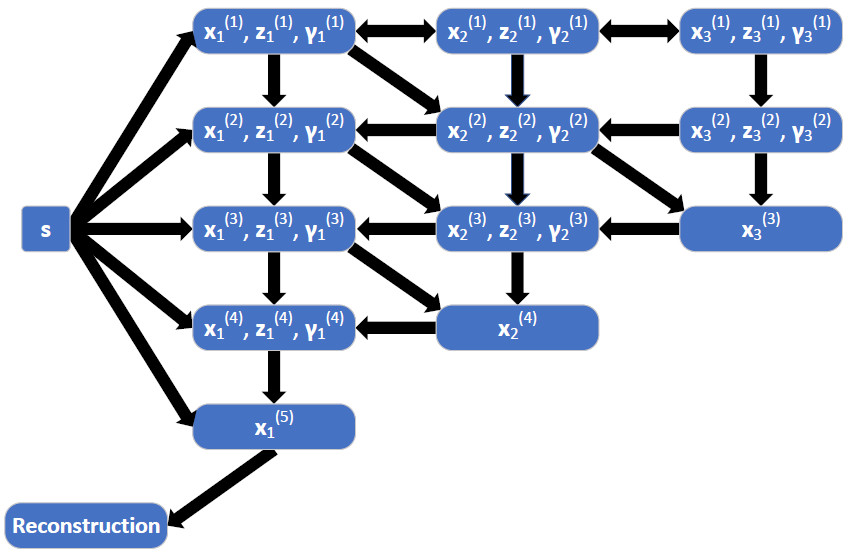
\includegraphics[width=\textwidth]{figures/multi-layer_ADMM-node-dependencies.PNG}
	\caption{This diagram shows interactions between layers across iterations. The double-sided arrows at the top of the diagram go both directions because $\vx_{\ell + 1}$ influences $\vz_{\ell}$ during initialization.}
	\label{figure:ADMM Multi-Layer Pursuit Diagram}
\end{figure}
\begin{algorithm}[h]
\SetAlgoLined 
\SetKwInOut{Input}{input}
\SetKwInOut{Output}{output}
\Input{Overrelaxation parameter: $\alpha \in (0,2]$, Number of layers: $L$, Number of filters: $M$, Signal size: $N$, Signal: $\vs$, Unnormalized dictionary for each layer: $\mD_{\ell}$, Objective function term coefficients: $\mu_{\ell}$ and $\lambda_{\ell}$, Efficient means to compute $(\rho\mId + \mD_{\ell}^T\mD_{\ell})^{-1}\vb$}
\Output{Sparse coding coefficients: either $\vx_{\ell}$ or $\vz_{\ell}$}
 %initialization:\\
   \For{$\ell \in \{1,\hdots, L\}$}
   {
      $\vgamma_{\ell} = \vzero$
      \For{$m \in \{1,\hdots, M\}$}
      {
         $r_{\ell}[m] = \|\mD_{\ell}[:,mN]\|_2$
      }
   }
   $\vx_1 = \mR_1^{-2} \mD_1^T$  \\
   \For{$\ell \in \{2,\hdots,L\}$}
   {
      $\vx_{\ell} = \mR_{\ell}^{-2}\mD_{\ell}^T\mR_{\ell - 1}\vx_{\ell - 1}$
   }
 \While{Not Converged}{
   \For{$\ell \in \{1,\hdots,L - 1\}$}
   {
      $\vz_{\ell} = (\rho\mu_{\ell}\mId + \mu_{\ell + 1}\mR_{\ell}^2)^{-1}\mR_{\ell}^2\operatorname{S}_{\lambda_{\ell}}\left(\mu_{\ell + 1}\mD_{\ell + 1}\vx_{\ell + 1} + \rho\mu_{\ell}\mR_{\ell}^{-1}(\vx_{\ell} - \vgamma_{\ell})\right)$
   }
   $\vz_L = \mR_L \operatorname{S}_{\frac{\lambda_L\mR_L}{\rho\mu_L}}(\vx_L - \vgamma_L)$ \\
   \For{$\ell \in \{1,\hdots,L\}$}
   {
      $\vgamma_{\ell} = \vgamma_{\ell} + \mR_{\ell}^{-1}\vz_{\ell} - \vx_{\ell}$
   }
   $\vx_1 = (\rho\mId + \mD_1^T\mD_1)^{-1}(\mD_1^T\vs + \rho(\mR_1^{-1}\vz_1 + \vgamma_1))$ \\
   \For{$\ell \in \{2,\hdots,L\}$}
   {
      $\vx_{\ell} = (\rho\mId + \mD_{\ell}^T\mD_{\ell})^{-1}(\mD_{\ell}^T\vz_{\ell - 1} + \rho(\mR_{\ell}^{-1}\vz_{\ell} + \vgamma_{\ell}))$
   }
   \For{$\ell \in \{1,\hdots,L\}$}
   {
      $\vgamma_{\ell} = \vgamma_{\ell} + (\alpha - 1)(\mR_{\ell}^{-1}\vz_{\ell} - \vx_{\ell})$
   }
 }
   \For{$\ell \in \{1,\hdots,L\}$}
   {
      $\vx_{\ell} = \mR_{\ell}\vx_{\ell}$
   }
 \caption{ADMM for Multi-Layer Pursuit with Unnormalized Dictionary}\label{algorithm:ADMM Multi-Layer Pursuit}
\end{algorithm}

\section{Dictionary Learning}
There are many possible approaches to compute dictionary updates, but the focus here will be on gradient descent. The pursuit algorithm generates several layers of coefficients from an input signal, and these coefficents can subsequently be used to generate some output, for classification, reconstruction, or some other task. With the appropriate choice of loss function $\loss$, backpropagation can be used to update the dictionaries. All of the computations in pursuit are almost\footnote{Like rectified linear activation functions, there is a discontinuity in the derivative for shrinkage operators. While such functions are technically not differentiable, this does not pose any issue for backpropagation. Operations that rely on a complex conjugate of a complex input also are not differentiable, but since the output is a scalar loss function, gradients can still be computed, which is sufficient for gradient descent. See Appendix C for details.} differentiable, so backpropagation is possible all the way back to the signal. Regardless of whether stochastic gradient descent or momentum methods such as Nesterov \cite{sutskever2013importance} or ADAM \cite{kingma2017adam} is used, the dictionary updates must be replaced with low-rank substitutes if the number of channels is large, so that the inverse decomposition can be updated efficiently. At least some of the gradients are computed in frequency domain. The convolutional filters are either spatially or temporally bound, and the frequency domain gradients will not respect that constraint, so they will need to be transformed and truncated.

Backpropagating gradients through most of the operations in the pursuit algorithm is very straightforward. Some platforms such as PyTorch \cite{paszke2017automatic} or TensorFlow \cite{tensorflow} will even do so automatically. However, the $\vx$-updates rely on a matrix decomposition to solve an inverse problem, and this prevents automatic differentiation in respect to the dictionaries. The equations necessary to compute gradients for the inverse problem in the $\vx$-update are derived in appendix C.
Let $\hat{\mD}_{\ell}$ be the frequency domain representation of the unnormalized dictionary corresponding to the $\ell$th layer, and let $\mQ_{\ell} = \rho\mId + \hat{\mD}_{\ell}^H\hat{\mD}_{\ell}$.
\begin{equation}
\nabla_{\hat{\mD}_{\ell}}^{(\vb \rightarrow \mQ_{\ell}^{-1}\vb)} \loss = -(\hat{\mD}_{\ell}\mQ_{\ell}^{-1}\vb)(\mQ_{\ell}^{-1}\nabla_{\mQ_{\ell}^{-1}\vb} \loss)^H - (\hat{\mD}_{\ell}\mQ_{\ell}^{-1}\nabla_{\mQ_{\ell}^{-1}\vb} \loss) (\mQ_{\ell}^{-1}\vb)^H
\end{equation}
where $\vb$ is the input vector to the computational step $\mQ_{\ell}^{-1}\vb$.\footnote{$\vb$ would take on a value like $\vb = \F\left((\mD_{\ell}\mR_{\ell})^T\vz_{\ell - 1}^{(t)} + \rho \left(\mR_{\ell}^{-1}\vz_{\ell}^{(t)} + \frac{\vgamma_{\ell}^{(t)}}{\rho\sqrt{\mu_{\ell}}}\right)\right) $, as seen in the $\vx$-update equation \ref{equation:Multi-Layer x-Update Equation}.} The superscript of the gradient specifies which gradient term is being computed. This is necessary because same dictionary gets reused across multiple computations, and so these gradient terms must be computed separately and then aggregated to get the actual gradient.

For the Woodbury form\footnote{Useful if the number of filters is larger than the number of channels}, the decomposition represents a different matrix for efficiently solving the inverse problem, and so the equation for the corresponding gradient term is different.
Let $\mXi_{\ell} = \rho\mId + \hat{\mD}_{\ell}\hat{\mD}_{\ell}^H$.
\begin{equation}
\nabla_{\hat{\mD}_{\ell}}^{(\vb \rightarrow \mXi_{\ell}^{-1}\vb)} \loss = -(\mXi_{\ell}^{-1}\nabla_{\mQ_{\ell}^{-1}\vb} \loss)(\hat{\mD}_{\ell}^H\mXi_{\ell}^{-1}\vb)^H -  (\mXi_{\ell}^{-1}\vb)(\hat{\mD}_{\ell}^H\mXi_{\ell}^{-1}\nabla_{\mQ_{\ell}^{-1}\vb} \loss)^H
\end{equation}
where $\vb$ is the input vector to the computational step $\mXi_{\ell}^{-1}\vb$.

With these equations it is possible to compute dictionary updates through backpropagation.  Putting it all together, a dictionary learning algorithm for multi-layer dictionary models is shown in algorithm \ref{algorithm:Multi-Layer Dictionary Learning}.

\begin{algorithm}[h]
\SetAlgoLined
   \SetKwInOut{Input}{input}
   \SetKwInOut{Output}{output}
   \Input{Overrelaxation Parameter: $\alpha \in (0,2]$, Signal: $\vs$, Unnormalized initial dictionary for each layer: $\mD_{\ell}$, Objective function term coefficients for each layer: $\mu_{\ell}$ and $\lambda_{\ell}$}
   \Output{Unnormalized dictionaries for each layer: $\mD_{\ell}$}
 %initialization:\\
   \For{$\ell \in \{1,\hdots,L\}$}
   {
      $\left(\rho\mId + \mD_{\ell}^T\mD_{\ell}\right) = \operatorname{ComputeDecomp}\left(\rho,\mD_{\ell} \right)$
   }
   $i = 0$ \\
   \While{Stopping Criteria Not Met}{
   $\vs = \operatorname{GetData}(i)$ \\
   $i = i + 1$ \\
   $\vx_1,\hdots,\vx_L = \operatorname{MultiLayerPursuit}(\vs,\alpha,\vmu,\vlambda,\mD,(\rho\mId + \mD_1^T\mD_1),\hdots,(\rho\mId + \mD_L^T\mD_L))$ \\
   $\loss = \operatorname{ComputeLoss}(\vx_1,\hdots,\vx_L)$ \\
   $\nabla_{\hat{\mD}_1} \loss,\hdots,\nabla_{\hat{\mD}_L} \loss = \operatorname{Backpropagation}(\loss,\mD_1,\hdots,\mD_L)$ \\
   $\mDelta \hat{\mD}_1,\hdots,\mDelta \hat{\mD}_L = \operatorname{CalculateGradientStep}(\nabla_{\hat{\mD}_1} \loss,\hdots,\nabla_{\hat{\mD}_L} \loss)$ \\
   \For{$\ell \in \{1,\hdots,L\}$}
   {
      $\tilde{\mD} = \operatorname{Normalize}(\hat{\mD}_{\ell} + \mDelta \hat{\mD}_{\ell})$ \\
      $\mDelta \mD_{\ell} = \operatorname{Truncate}(\F^{-1}\operatorname{RandomizedSVD}(\tilde{\mD} - \hat{\mD}_{\ell}))$ \\
      $\left(\rho\mId + \mD_{\ell}^T\mD_{\ell}\right) = \operatorname{UpdateDecomp}\left(\left(\rho\mId + \mD_{\ell}^T\mD_{\ell}\right),\rho,\mD_s,\mDelta\mD \right)$ \\
      $\mD_{\ell} = \mD + \mDelta\mD$ \\
      $\hat{\mD}_{\ell} = \F(\mD_{\ell})$
   }
   }
 \caption{Multi-Layer Dictionary Learning}\label{algorithm:Multi-Layer Dictionary Learning}
\end{algorithm}

\section{Summary}
In this chapter, I have applied the novel sparse coding algorithm from the previous chapter to a multi-layer dictionary model. If the dictionaries are updated with low-rank updates, the inverse representation necessary for the $\vx$ updates in the algorithm can be updated efficiently. This approach offers an alternative to direct proximal methods such as FISTA or mathematically suspect inverse approximations like the tight-frame assumption.


%%%%%%%%%%%%%%%%
% Chapter 4
%%%%%%%%%%%%%%%%

\chapter{JPEG Artifact Removal}
\section{Introduction}
Despite the existance of better compression algorithms, use of the JPEG compression algorithm is ubiquitous: it is the most commonly used image compression algorithm.  Overzealous JPEG compression can produce visible distortions, and image restoration from these distortions is a challenging problem. There are two aspects of JPEG compression which make the restoration process more challenging than simpler restoration problems like deblurring or removing salt-and-pepper noise: JPEG's block-based approach is not spatially invariant, and the quantization is nonlinear. This chapter describes a novel approach to address the challenges of JPEG image restoration using the ADMM-based convolutional sparse coding for a multi-layer dictionary model.
\section{JPEG Algorithm}

The JPEG compression process begins with an RGB image input, and consists of five steps. The first is a color transformation, transitioning from RGB to YUV. Then, the U and V color channels are downsampled.  The DCT for each $8 \times 8$ block is computed (separately for each channel).  The DCT coefficients are then quantized using a quantization matrix determined by a user-chosen JPEG quality factor. Finally, these quantized coefficients are reodered and encoded using a lossless variable length coding process.

The standard reconstruction process reverses the lossless encoding, computes the IDCT of the blocks, upsamples the color channels, and reverses the color transform.
\section{Literature Review}
\section{Modelling Compressed JPEG Images}
Some researchers have observed convolutional dictionary models struggle with large smooth components of signals, likely due to the fact that shifted versions of smooth filters have high coherence.

For this reason, it is often a good idea to subtract a smoothed version $\vs_{\text{smth}}$ of the signal, and only apply apply the dictionary model to the residual $\vs_{\text{rough}}$.

\begin{equation}
\vs_{\text{clean}} = \vs_{\text{smth}} + \vs_{\text{rough}}
\end{equation}

\begin{equation}
\vs_{\text{rough}} \approx \mD_1\vx_1
\end{equation}

When restoring an image after JPEG compression, the original image $\vs_{\text{clean}}$ is not known. Instead, the compressed image $\vs$ is observed.

\begin{equation}
\vs = \mQ\mW\vs_{\text{clean}}
\end{equation}

\begin{equation}
\vs \approx \mQ\mW(\vs_{\text{smth}} + \mD_1\vx_1)
\end{equation}

where $\mW$ maps the signal to $8 \times 8$ block frequency coefficients (from the cosine transform), and $\mQ$ quantizes them.

A means of estimating $\vs_{\text{smth}}$ from JPEG-compressed image $\vs$ is discussed in the Practical Considerations chapter.

From this idea, I construct the pursuit problem:
\begin{equation}
\begin{aligned}
\minimize_{\vx} & \frac{\mu_1}{2}\|\vs - \mQ\mW(\mD_1\vx_1 + \vs_{\text{smth}})\|_2^2 + \sum_{\ell = 2}^L \frac{\mu_{\ell}}{2}\|\vx_{\ell - 1} - \mD_{\ell}\vx_{\ell}\|_2^2 + \sum_{\ell = 1}^L \lambda_{\ell}\|\vx_{\ell}\|_1 \\
\text{subject to } & \vx_{\ell} > \vzero
\end{aligned}
\end{equation}

with $\lambda_{\ell} \geq \vzero$.

My approach to solve this problem uses the ADMM algorthm, where $\vx_1,\ldots,\vx_L$ are the first set of primal variables, $\vv,\vz_1,\ldots,\vz_L$ are the second set of primal variables,  and $\vgamma_1,\ldots,\vgamma_L$ are the dual variables corresponding to contraints on $\vz_1,\ldots,\vz_L$.  Here is the corresponding optimization problem:

\begin{equation}
\begin{aligned}
\minimize_{\vx,\vv,\vz} & \frac{\mu_1}{2}\|\vv - \mD_1\vx_1  - \vs_{\text{smth}}\|_2^2 + \sum_{\ell = 2}^L \frac{\mu_{\ell}}{2}\|\vz_{\ell - 1} - \mD_{\ell}\vx_{\ell}\|_2^2 + \sum_{\ell = 1}^L \lambda_{\ell}\|\vz_{\ell}\|_1 \\
\text{subject to } & \sqrt{\mu}\mR_{\ell}^{-1}(\vz_{\ell} - \vx_{\ell}) = \vzero \\
                   & \mQ\mW(\vv) - \vs = \vzero
\end{aligned}
\end{equation}

The constraint $\mQ\mW(\vv) - \vs = \vzero$ is not an affine constraint because of the quantization. To resolve this, \cite{chodosh2020use}) approximate the quantization as a linear operator. However, the constraint is convex, so the constraint can be handled without approximation implicitly using and indicator function. For now, I will focus on the other variable updates.

Setting $\vz_0 = \vv - \vs_{\text{smth}}$, the updates for $\vx$, $\vz$, and $\vgamma$ are identitical to those from the last chpater.

\begin{equation}
\mR_{\ell}^{-1}\vx_{\ell}^{(t + 1)} = \left(\rho \mId + (\mD_{\ell}\mR_{\ell})^T\mD_{\ell}\mR_{\ell}\right)^{-1}\left((\mD_{\ell}\mR_{\ell})^T\vz_{\ell - 1}^{(t)} + \rho \left(\mR_{\ell}^{-1}\vz_{\ell}^{(t)} + \frac{\vgamma_{\ell}^{(t)}}{\rho\sqrt{\mu_{\ell}}}\right)\right)
\end{equation}

\begin{equation}
\vz_{\ell}^{(t + 1)} = (\rho\mu_{\ell}\mId + \mu_{\ell + 1}\mR_{\ell}^2)^{-1}\mR_{\ell}^2\operatorname{S}_{\lambda_{\ell}}\left(\mu_{\ell + 1}\mD_{\ell + 1}\vx_{\ell + 1}^{(t + 1)} + \rho\mu_{\ell}\mR_{\ell}^{-1}\left(\mR_{\ell}^{-1}\vx_{\ell}^{(t + 1)} - \frac{\vgamma_{\ell}^{(t + \frac{1}{2})}}{\rho\sqrt{\mu_{\ell}}}\right)\right)
\end{equation}

\begin{equation}
\vz_L^{(t + 1)} = \mR_{\ell}\operatorname{S}_{\frac{\lambda_L\mR_L}{\rho\mu_L}}\left(\mR_L^{-1}\vx_L^{(t + 1)} - \frac{\vgamma_L^{(t + \frac{1}{2})}}{\rho\sqrt{\mu_L}}\right)
\end{equation}

\begin{equation}
\frac{\vgamma_{\ell}^{\left(t + \frac{1}{2}\right)}}{\rho\sqrt{\mu_{\ell}}} = \frac{\vgamma_{\ell}^{(t)}}{\rho\sqrt{\mu_{\ell}}} + (\alpha - 1)(\mR_{\ell}^{-1}\vz_{\ell}^{(t)} - \mR^{-1}\vz_{\ell}^{(t + 1)})
\end{equation}

\begin{equation}
\frac{\vgamma_{\ell}^{(t + 1)}}{\rho\sqrt{\mu_{\ell}}} = \frac{\vgamma_{\ell}^{\left(t + \frac{1}{2}\right)}}{\rho\sqrt{\mu_{\ell}}} + \mR_{\ell}^{-1}\vz_{\ell}^{(t + 1)} - \mR^{-1}\vz_{\ell}^{(t + 1)} 
\end{equation}


The only remaining update equation is for $\vv$. This deals with the non-affine constraint, which complicates the problem. I will present a method for handling the quantization operator in the constraint in the next section.

\section{Handling Quantization}



Recall the optimization problem:
\begin{equation}
\begin{aligned}
\minimize_{\vx,\vv,\vz} & \frac{\mu_1}{2}\|\vv - \mD_1\vx_1  - \vs_{\text{smth}}\|_2^2 + \sum_{\ell = 2}^L \frac{\mu_{\ell}}{2}\|\vz_{\ell - 1} - \mD_{\ell}\vx_{\ell}\|_2^2 + \sum_{\ell = 1}^L \lambda_{\ell}\|\vz_{\ell}\|_1 \\
\text{subject to } & \sqrt{\mu}\mR_{\ell}^{-1}(\vz_{\ell} - \vx_{\ell}) = \vzero \\
                   & \mQ(\mW\vv) - \vs = \vzero
\end{aligned}
\end{equation}


For the $\vv$ update, it is helpful to introduce a common convex-optimization trick. Consider the following function:
\begin{equation}
\indicator_{\{\mQ\mW(\vv) - \vs = \vzero\}} = \begin{cases} 0 & \mQ(\mW\vv) - \vs = \vzero \\ + \infty & \text{otherwise} \end{cases}
\end{equation}

The function is convex, and when included in an objective function, it implicitly enforces the constraint $\mQ(\mW\vv) - \vs = \vzero$ This can be rewritten as the following:\footnote{The set $\{\vv: \mQ(\mW\vv) - \vs = \vzero\}$ does not include all boundary points. Equation \ref{equation:Indicator} uses the closure of the set instead. This ensures that there is a minimizer of the augmented Lagrangian in respect to $\vv$.} 

\begin{equation} \label{equation:Indicator}
\indicator_{\{\mQ(\mW\vv) - \vs = \vzero\}} = \begin{cases} 0 & \vs - \frac{\vq}{2} \leq \mW\vv \leq \vs + \frac{\vq}{2} \\ + \infty & \text{otherwise} \end{cases}
\end{equation}

Adding the indicator function to the objective produces the following Lagrangian function: 

\begin{equation}
\begin{split}
\L_{\rho}(\vx,\vv,\vz,\veta,\vgamma) =  \frac{\mu_1}{2}\|\vv - \mD_1\vx_1  - \vs_{\text{smth}}\|_2^2 + \psi(\vx,\vz,\vgamma) + \indicator_{\{\mQ(\mW\vv) - \vs = \vzero\}}
\end{split}
\end{equation}

where $h\psi(\vx,\vz,\vgamma)$ is a collection of terms irrelevant to the updates for $\vv$.

Handling the cases in pointwise fashion, define function $h$ as the following clipping operation:


\begin{equation}
\operatorname{h}(\vx_1) = \mW(\vv - \mD_1\vx_1 - \vs_{\textrm{smth}}) = \begin{cases} \vs + \frac{\vq}{2} - \mW(\mD_1\vx_1 + \vs_{\textrm{smth}}) & \mW(\mD_1\vx_1 + \vs_{\textrm{smth}}) > \vs + \frac{\vq}{2} \\ \vs - \frac{\vq}{2} - \mW(\mD_1\vx_1 + \vs_{\textrm{smth}}) & \mW(\mD_1\vx_1) + \vs_{\textrm{smth}}) < \vs - \frac{\vq}{2} \\ \vzero & \text{otherwise}
\end{cases}
\end{equation}

Then,
\begin{equation}
\vv^{(t + 1)} = \mD_1\vx_1^{(t + 1)} + \vs_{\text{smth}} + \mW^{\dagger}\operatorname{h}(\vx_1^{(t + 1)})
\end{equation}
where $\mW^{\dagger}$ is the pseudo-inverse of $\mW$.


\section{Experiment}
In this section, I apply this novel multi-layer dictionary approach to other multi-layer dictionary algorithms on the task of removing artifacts from JPEG compression.
\subsection{Experiment Setup}
The BSDS500 dataset consists of $200$ training images, $100$ validation images, and $200$ test images, and was originally designed to test segmentation algorithms. For this experiment, I compress the images using a quality factor of $25$. For training, the algorithms are given both the compressed and uncompressed images. The images vary in size, so I split the images into smaller $32 \times 32$ patches. For validation and testing, the algorithms are assessed on how well they reconstruct original image patches from the compressed image patches.
\subsection{Results}
My code is still running, so I do not have results to share yet.  I intend to compare to a proximal algorithm like \cite{chodosh2020use} or FISTA, single-layer ADMM, and the tight-frame approximation for the inverse problem.
\section{Conclusion}
It is hard to reach conclusions until my code is finished, but I am hopeful that my approach will be a competitive alternative to FISTA, and outperform single-layer ADMM and tight-frame approximations.


%%%%%%%%%%%%%%%%
% Chapter 5
%%%%%%%%%%%%%%%%

\chapter{Practical Considerations Concerning Tensorflow}
\section{Boundary Handling}

\section{Removing Low-Frequency Signal Content}

\subsection{JPEG Artifact Removal}

\section{Tensorflow and Keras}
Most of the computations for my research rely on TensorFlow version 2.3.1 \cite{tensorflow}, a Python library for machine learning specializing in building models with differentiable, parameterizable composite functions and learning model parameters using gradient descent or other gradient-based optimization methods. TensorFlow is a common platform for researchers and developers working on artificial neural netwokrs, and there are many tutorials and exampes freely available online, so I will not replicate that work here. This chapter section the reader already has some familiarity with TensorFlow and Keras \cite{keras} (a high-level library inside TensorFlow). The goal of this section is to provide the reader with the tools and workarounds to be able to replicate my work without resorting to hacking things together with gradient tape and/or TensorFlow-1-style code.

\subsection{Why Not Use Gradient Tape and TensorFlow-1-Stye Code?}
Keras offers a high-level environment. Code written in Keras's framework is easier to integrate with other work. Gradient tape is great for hacking something together or debugging, but promotes styles of coding that are less readable, less maintainable, and less portable. Keras also has a lower learning curve than the broader TensorFlow library.
\TODO{I should write more for this section or possibly remove it. Might help to read through Keras documentation and endorsements to see why they think it's necessary.}


\subsection{Shared Weights Between Layers}
Trainable TensorFlow variables declared outside of any Keras layer will not be automatically added to a Keras model's list of trainable variables. In most cases, this limitation is not a problem; it is intuitive to declare a layer's weights inside that layer. However, sometimes the same variable is needed in multiple distinct layers. To be include a variable in the model's trainable variables, it is sufficient to declare the variable in one layer and pass the variable (or the layer it was initialized in) as an input argument to the \_\_init\_\_ function of the other layers that share that variable. This will work even if the Keras model does not use the layer that declared the variable. \footnote{One could instead declare the variable outside any layers, pass it into the \_\_init\_\_ functions of all the variables that depend on it, and then manually add the variable to the model's list of trainable variables, but I do not recommend this approach. The resulting code will be less readable and much less maintainable.}

\subsection{Custom Partial Gradients}
TensorFlow offers a well-documented means of replacing TensorFlow's gradient computations of an operation with specified custom gradient computations. However, if the operation involves multiple tensors that are inputs or trainable variables, the standard approach replaces all the gradients with custom gradients. If TensorFlow's gradient computations are sufficient for some tensors but not others, a workaround is necessary. This workaround is best explained by example.

Suppose the operation is the following:


\begin{code}
z = f(x,y)
\end{code}

for which the standard TensorFlow gradient computations of $f$ are desired in respect to $x$, but the custom gradient computations desired in respect to $y$ are specified in function $g(\nabla_z \L)$. This can be rewritten as the following:

\begin{code}
@tf.custom_gradient
def h(z,y):
    def grad_fun(grad):
        return (tf.identity(grad),g(grad))
    return z,grad_fun
z = f(x,tf.stop_gradient(y))
z = h(z,y)
\end{code}

The function $h$ does nothing on the forward pass, but in the backward pass computes the custom gradient in respect to $y$ as intended.

\subsection{Updating TensorFlow Variables After Applying Gradients}
To update TensorFlow Variables after applying gradients, it is necessary to track which variables are affected and what their corresponding update functions are. To accomplish this, I store the update functions in a Python dictionary using variable names as the dictionary keys. This Python dictionary needs to be widely accessible so that layers can add update functions when they are initialized; a simple way to do this is to make the update function Python dictionary a class attribute. The keys need to be unique, but TensorFlow variable names can conflict. It is easy to avoid this problem by checking for conflicts before adding a new update function.

\begin{code}
class PostProcess:
    update = {}
    def add_update(varName,update_fun):
        assert varName not in PostProcess.update
        PostProcess.update[varName] = update_fun
\end{code}


In the standard Keras training paradigm, models are trained using the fit function, a method in the Keras model object. The fit function calls the function train\_step, where gradients are applied.  To update TensorFlow Variables after gradients are applied, train\_step is the function to modify. The only change that needs to be made is adding a function call to all update functions that correspond to the model's list of trainable variables.

\begin{code}
class Model_subclass(tf.keras.Model):
    def train_step(self,data):
        trainStepOutputs = tf.keras.Model.train_step(self,data)
        update_ops = []
        for tv in self.trainable_variables:
            if tv.name in PostProcess.update:
                PostProcess.update[tv.name]()
        return trainStepOutputs
\end{code}

Changes to Tensorflow variables in the update function must use the assign command (or its variants: assign\_add, assign\_sub, ect). Otherwise, TensorFlow will detect that computations lie outside of its computational graph and throw an error. Note that using the assign command on Python variables that are not TensorFlow variables will produce some very cryptic error messages, so be sure to use the assign command correctly. If the value change of one TensorFlow variable depends on the value of another TenorFlow variable value pre-update, it may be necessary to use the Tensorflow control\_dependencies command to get TensorFlow to track that dependency. TensorFlow has a useful tool called TensorBoard that helps visualize TensorFlow's dependencies, but a workaround is required to use TensorBoard on update functions that are called after applying gradients. To use TensorBoard to visualize dependencies in an update function, temporarily call the update function in the layer's call method, use TensorBoard to verify all necessary dependancies are being tracked, then remove the update function call from the layer's call method.

\subsection{The Perils of Using Built-In Functions for Complex Tensors and Arrays}
The TensorFlow Probability version 0.11.1 \cite{tensorflowprobability} is an extension of TensorFlow mosly used for probabilistic models. The library contains a Cholesky update function, but the function does not properly handle complex inputs. To compute Cholesky updates for complex inputs, users should either write their own implementation or use my code (included in supplementary material). Similarly, the Randomized SVD algorithm in the Python scikit-learn library does not properly handle complex inputs.

Errors like these are fairly common, so when dealing with complex data, researchers and practitioners should carefully verify that the function libraries they rely on are properly handling complex numbers.


%%%%%%%%%%%%%%%%
% Chapter 6
%%%%%%%%%%%%%%%%



%%%%%%%%%%%%%%%%
% Chapter 7
%%%%%%%%%%%%%%%%

%%%%%%%%%%%%%%%%
% Conclusion
%%%%%%%%%%%%%%%%

\chapter{Conclusion}
This dissertation has presented a novel dictionary learning algorithm for signals with a large number of channels and its application to multi-layer dictionary models. This algorithm can be used for JPEG artifact removal, and shows some promise as a competitor to the FISTA algorithm, given its faster convergence in solving the sparse-coding problem, but does have larger memory requirements than FISTA. In addition, appendix A generalizes the work of \cite{krause2015more} to handle complex numbers, which to my knowledge has not been done previously. \cite{krause2015more} efficiently computes rank-$1$ updates for a Cholesky factorization.

In addition to seeking other applications, future expansion on this research might look to adapt $\rho$ during training. While $\rho$ must remain fixed for efficient updates of the Cholesky decomposition (or LDLT decomposition), drift over many iterations eventually must be rectified by recomputing the entire decomposition. At such time, an update to $\rho$ would require no additional computational cost. While many methods exist to adapt $\rho$ for ADMM \cite{he2000alternating}\cite{xu2017adaptive}, these methods are designed to adjust $\rho$ far more frequently. Another potential area of future research lies in tailoring momentum methods for dictionary updates to this novel dictionary learning algorithm. While the dictionary learning algorithm is not incompatible with momentum-based dictionary updates, conventional momentum methods \cite{sutskever2013importance}\cite{kingma2017adam} will not take into account the low-rank approximation step, which may hurt performance. Finally, since the memory requirements promote the use of frames to decrease the signal size, there may be a need in some applications to combine results across frames. Fortunately, given the popularity of frame-based dictionary models, there is an existing body of work to build off of for this task \cite{elad2006image}\cite{yang2010image}\cite{turquais2017method}\cite{jiang2021combining}.


%%%%%%%%%%%%%%%%
% Appendices
%%%%%%%%%%%%%%%%

\begin{appendices}

%Some Table of Contents entry formatting
\addtocontents{toc}{\protect\renewcommand{\protect\cftchappresnum}{\appendixname\space}}
\addtocontents{toc}{\protect\renewcommand{\protect\cftchapnumwidth}{6em}}

%Begin individual appendices, separated as chapters

\chapter{Cholesky Hermitian Rank-1 Updates}
These derivations are based on the work of \cite{krause2015more}, but modified to handle complex numbers.


Let $\mA^{(n)} = \mL\mL^H$ be a Hermitian, positive definite matrix of dimension $C \times C$ and $\mL$ be a lower trangular matrix. Then, the diagonal of $\mL$ is positive and real.

\begin{equation}
\mA^{(n)} = \begin{bmatrix} a_{1,1} & \hdots & a_{C,1}^{*} \\
                      \vdots & \ddots & \vdots \\
                      a_{C,1} & \hdots & a_{C,C}
      \end{bmatrix}
\end{equation}

\begin{equation}
\mL = \begin{bmatrix} \ell_{1,1} & 0      & \hdots & 0 \\
                      \ell_{2,1} & \ddots &        & \vdots \\
                      \vdots     &        &  \ddots &  0     \\
                      \ell_{C,1}     & \hdots &   & \ell_{C,C}
      \end{bmatrix}
\end{equation}

Dividing $\mA^{(n)}$ into blocks:
\begin{equation}
\mA^{(n)} = \begin{bmatrix}\ell_{1,1} & \vzero^T \\ \vl_{2,1} & \mL_{2,2} \end{bmatrix} \begin{bmatrix} \ell_{1,1}^{*} & \vl_{2,1}^H \\ \vzero & \mL_{2,2}^H \end{bmatrix} 
\end{equation}

\begin{equation}
\mA^{(n)} = \begin{bmatrix} \ell_{1,1}^2 & \ell_{1,1}\vl_{2,1}^H \\ \ell_{1,1}\vl_{2,1} & \mL_{2,2}\mL_{2,2}^H + \vl_{2,1}\vl_{2,1}^H \end{bmatrix}
\end{equation}

Consider the rank-$1$ update:\footnote{If $\lambda$ is negative, the result is not guarenteed to be positive definite. In general, updates to inverse representations with a negative $\lambda$ (sometimes refered to as "downdates") are less numerically stable, even if the resulting matrix is still positive definite.}
\begin{equation}
\mA^{(n + 1)} = \mA^{(n)} + \lambda\vv\vv^H
\end{equation}

where
\begin{equation}
\vv = \begin{bmatrix} v_1 \\ \vv_2 \end{bmatrix}
\end{equation}

\begin{equation}
\mA^{(n + 1)} = \begin{bmatrix} \ell_{1,1}^2 + \lambda v_1 v_1^{*} & \ell_{1,1}\vl_{2,1}^H + \lambda v_1\vv_2^H \\ \ell_{1,1}\vl_{2,1} + \lambda v_1^{*}\vv_2 & \mL_{2,2}\mL_{2,2}^H + \vl_{2,1}\vl_{2,1}^H + \lambda\vv_2\vv_2^H \end{bmatrix}
\end{equation}

Let $\mA^{(n + 1)} = \mM\mM^H$, where $\mM$ is a lower triangular matrix. Then, the diagonal of $\mM$ is positive and real.

\begin{equation}
\mA^{(n + 1)} = \begin{bmatrix} m_{1,1}^2 & m_{1,1}\vm_{2,1}^H \\ m_{1,1}\vm_{2,1} & \mM_{2,2}\mM_{2,2}^H + \vm_{2,1}\vm_{2,1}^H \end{bmatrix}
\end{equation}

Therefore,
\begin{equation}
m_{1,1}^2 = \ell_{1,1}^2 + \lambda v_1 v_1^{*}
\end{equation}
\begin{equation}
m_{1,1}\vm_{2,1} = \ell_{1,1}\vl_{2,1} + \lambda v_1^{*}\vv_2
\end{equation}
\begin{equation}
\mM_{2,2}\mM_{2,2}^H + \vm_{2,1}\vm_{2,1}^H = \mL_{2,2}\mL_{2,2}^H + \vl_{2,1}\vl_{2,1}^H + \lambda\vv_2\vv_2^H
\end{equation}

Solving for the first column of $\mM$:
\begin{equation} \label{equation:m11}
m_{1,1} = \sqrt{\ell_{1,1}^2 + \lambda v_1 v_1^{*}}
\end{equation}
\begin{equation}
\vm_{2,1} = \frac{\ell_{1,1}\vl_{2,1} + \lambda v_1^{*}\vv_2}{m_{1,1}}
\end{equation}
Finally,
\begin{equation}
\mM_{2,2}\mM_{2,2}^H = \mL_{2,2}\mL_{2,2}^H + \vl_{2,1}\vl_{2,1}^H + \lambda\vv_2\vv_2^H - \vm_{2,1}\vm_{2,1}^H
\end{equation}

\begin{equation}
\vm_{2,1}\vm_{2,1}^H = \frac{1}{m_{1,1}^2}\left(\ell_{1,1}^2\vl_{2,1}\vl_{2,1}^H + \lambda\ell_{1,1}v_1\vl_{2,1}\vv_2^H + \lambda\ell_{1,1}v_1^{*}\vv_2\vl_{2,1}^H + \lambda^2 v_1 v_1^{*} \vv_2\vv_2^H\right)
\end{equation}

\begin{equation}
\mM_{2,2}\mM_{2,2}^H = \mL_{2,2}\mL_{2,2}^H + \frac{m_{1,1}^2 - \ell_{1,1}^2}{m_{1,1}^2}\vl_{2,1}\vl_{2,1}^H + \frac{\lambda(m_{1,1}^2 - \lambda v_1 v_1^{*})}{m_{1,1}^2}\vv_2\vv_2^H - \frac{\lambda\ell_{1,1}v_1}{m_{1,1}^2}\vl_{2,1}\vv_2^H - \frac{\lambda\ell_{1,1}v_1^{*}}{m_{1,1}}\vv_2\vl_{2,1}^H
\end{equation}

The expressions $m_{1,1}^2 - \lambda v_1 v_1^{*}$ and $m_{1,1}^2 - \ell_{1,1}^2$ can be simplified using equation \ref{equation:m11}.
\begin{equation}
\mM_{2,2}\mM_{2,2}^H = \mL_{2,2}\mL_{2,2}^H + \frac{\lambda v_1 v_1^{*} }{m_{1,1}^2}\vl_{2,1}\vl_{2,1}^H + \frac{\lambda \ell_{1,1}^2}{m_{1,1}^2}\vv_2\vv_2^H - \frac{\lambda\ell_{1,1}v_1}{m_{1,1}}\vl_{2,1}\vv_2^H - \frac{\lambda\ell_{1,1}v_1^{*}}{m_{1,1}^2}\vv_2\vl_{2,1}^H
\end{equation}

Factoring out $\frac{\lambda}{m_{1,1}^2}$:
\begin{equation}
\mM_{2,2}\mM_{2,2}^H = \mL_{2,2}\mL_{2,2}^H + \frac{\lambda}{m_{1,1}^2}\left( v_1 v_1^{*} \vl_{2,1}\vl_{2,1}^H + \ell_{1,1}^2\vv_2\vv_2^H - \ell_{1,1}v_1\vl_{2,1}\vv_2^H - \ell_{1,1}v_1^{*}\vv_2\vl_{2,1}^H\right)
\end{equation}

Note the factorization:
\begin{equation}
(\ell_{1,1}\vv_2 - v_1\vl_{2,1})(\ell_{1,1}\vv_2 - v_1\vl_{2,1})^H = \ell_{1,1}^2\vv_2\vv_2^H - \ell_{1,1}v_1^{*}\vl_{2,1}^H - \ell_{1,1}v_1\vl_{2,1}\vv_2 + v_1 v_1^{*}\vl_{2,1}\vl_{2,1}^H
\end{equation}
Therefore,
\begin{equation}
\mM_{2,2}\mM_{2,2}^H = \mL_{2,2}\mL_{2,2}^H + \frac{\lambda}{m_{1,1}^2}\left(\ell_{1,1}\vv_2 - v_1\vl_{2,1}\right)\left(\ell_{1,1}\vv_2 - v_1\vl_{2,1}\right)^H
\end{equation}
$\mL_{2,2}\mL_{2,2}^H$ is a $ (C - 1) \times (C - 1)$ Hermitian, positive definite matrix and $\frac{\lambda}{m_{1,1}^2}(\ell_{1,1}\vv_2 - v_1\vl_{2,1})(\ell_{1,1}\vv_2 - v_1\vl_{2,1})^H$ is a rank-$1$ Hermitian update, so the process can be repeated on subsequent columns of $\mL$ until the entire Cholesky decomposition has been updated. Each column update is computed in linear time, so the entire update can be computed in quadratic time.

While the order of complexity cannot be further reduced, there are changes that can be made to decrease precision error. Factoring out $\ell_{1,1}$:
\begin{equation}
\mM_{2,2}\mM_{2,2}^H = \mL_{2,2}\mL_{2,2}^H + \frac{\lambda\ell_{1,1}^2}{m_{1,1}^2}\left(\vv_2 - \frac{v_1}{\ell_{1,1}}\vl_{2,1}\right)\left(\vv_2 - \frac{v_1}{\ell_{1,1}}\vl_{2,1}\right)^H
\end{equation}

Rather than directly updating $\lambda$ before moving on to the next column, better precision can be achieved by updating a divisor instead.  Looking at the fraction $\frac{\ell_{1,1}^2}{m_{1,1}^2}$:
\begin{equation}
\frac{\ell_{1,1}^2}{m_{1,1}^2} = \frac{\ell_{1,1}^2}{\ell_{1,1}^2 + \lambda v_1 v_1^{*}}
\end{equation}

\begin{equation}
\frac{\ell_{1,1}^2}{m_{1,1}^2} = \frac{1}{1 + \frac{\lambda v_1 v_1^{*}}{\ell_{1,1}^2}}
\end{equation}

Therefore,
\begin{equation}
\mM_{2,2}\mM_{2,2}^H = \mL_{2,2}\mL_{2,2}^H + \frac{\lambda}{1 + \frac{\lambda v_1 v_1^{*}}{\ell_{1,1}^2}}(\vv_2 - \frac{v_1}{\ell_{1,1}}\vl_{2,1})(\vv_2 - \frac{v_1}{\ell_{1,1}}\vl_{2,1})^H
\end{equation}

Let
\begin{equation}
\vomega = \vv_2 - \frac{v_1}{\ell_{1,1}}\vl_{2,1}
\end{equation}

So,
\begin{equation}
\mM_{2,2}\mM_{2,2}^H = \mL_{2,2}\mL_{2,2}^H + \frac{\lambda}{1 + \frac{\lambda v_1 v_1^{*}}{\ell_{1,1}^2}}\vomega\vomega^H
\end{equation}

I will now write $\vm_{2,1}$ in terms of $\vomega$. Recall that
\begin{equation}
\vm_{2,1} = \frac{\ell_{1,1}\vl_{2,1} + \lambda v_1^{*}\vv_2}{m_{1,1}}
\end{equation}

Substituting for $\vv_2$:
\begin{equation}
\vm_{2,1} = \frac{\ell_{1,1}\vl_{2,1} + \lambda v_1^{*}(\vomega + \frac{v_1}{\ell_{1,1}}\vl_{2,1})}{m_{1,1}}
\end{equation}

Combining the $\vl_{2,1}$ terms:
\begin{equation}
\vm_{2,1} = \frac{(\ell_{1,1} +  \frac{\lambda v_1 v_1^{*}}{\ell_{1,1}}) \vl_{2,1} + \lambda v_1^{*}\vomega}{m_{1,1}}
\end{equation}

Factoring out $\frac{1}{\ell_{1,1}}$ produces the expression for $m_{1,1}^2$.
\begin{equation}
\vm_{2,1} = \frac{\frac{1}{\ell_{1,1}}(\ell_{1,1}^2 +  \lambda v_1 v_1^{*}) \vl_{2,1} + \lambda v_1^{*}\vomega}{m_{1,1}}
\end{equation}
\begin{equation}
\vm_{2,1} = \frac{\frac{m_{1,1}^2}{\ell_{1,1}} \vl_{2,1} + \lambda v_1^{*}\vomega}{m_{1,1}}
\end{equation}

\begin{equation}
\vm_{2,1} = \frac{m_{1,1}}{\ell_{1,1}} \vl_{2,1} + \frac{\lambda v_1^{*}}{m_{1,1}}\vomega
\end{equation}

So, to summarize:
\begin{equation} \label{equation:m11}
m_{1,1} = \sqrt{\ell_{1,1}^2 + \lambda |v_1|^2}
\end{equation}

\begin{equation}
\vomega = \vv_2 - \frac{v_1}{\ell_{1,1}}\vl_{2,1}
\end{equation}

\begin{equation}
\vm_{2,1} = \frac{m_{1,1}}{\ell_{1,1}} \vl_{2,1} + \frac{\lambda v_1^{*}}{m_{1,1}}\vomega
\end{equation}

\begin{equation}
\mM_{2,2}\mM_{2,2}^H = \mL_{2,2}\mL_{2,2}^H + \frac{\lambda}{1 + \frac{\lambda |v_1|^2}{\ell_{1,1}^2}}\vomega\vomega^H
\end{equation}

The rank-$1$ Hermitian update to a Cholesky decomposition can be computed in quadratic time. 


\chapter{Rank-2 Eigendecomposition Edge Cases}

\section{Less than 2 Independent Eigenvectors}

\begin{equation}
\mB = \begin{bmatrix} \mD^H\vu & \vv\end{bmatrix}^H
\end{equation}


The matrix $\mA\mB$ is a Hermitian $M \times M$ matrix, so it has $M$ real eigenvalues and $M$ independent eigenvectors which can be chosen to be orthogonal. Therefore, $\mB\mA$ has $2$ independent eigenvectors if $\mB$ is rank $2$.  There are three cases that can cause $\mB$ to have a rank less than $2$.


\begin{enumerate}
\item
\begin{equation}
\mD^H\vu = \vzero
\end{equation}
\item

\begin{equation}
\vv = \vzero
\end{equation}
\item
\begin{equation}
\mD^H\vu = \alpha \vv
\end{equation}
\end{enumerate}

In the first $2$ cases, the matrix $\mB\mA$ has one independent eigenvector. The first case implies that only the Hermitian update is nonzero.  The second case implies that the entire update is zero. (The eigenvalues are zero, so as long as the normalization of eigenvectors is handled with care, it is not necessary to check for these cases in code.)

In the third case, the diagonalization of $\mA\mB$ can be determined directly without using the $2 \times 2$ matrix $\mB\mA$.

\begin{equation}
\mA\mB = 2\operatorname{real}(\alpha)\vv\vv^H
\end{equation}

\begin{equation}
\lambda = 2\operatorname{real}(\alpha) \|\vv\|_2^2
\end{equation}

\begin{equation}
\vx = \frac{\vv}{\|\vv\|_2}
\end{equation}

The rest of the eigenvalues are zero.  (The corresponding $2 \times 2$ matrix $\mB\mA$ shares the same nonzero eigenvalue. The eigenvector that is lost has an eigenvalue of zero, so like in the other $2$ cases, it is not necessary to check for this case in code.)

\section{Eigenvalues are Not Distinct}

If the pair of eigenvalues are the same, then all nonzero vectors are eigenvectors of $\mB\mA$. However, it is necessary for a diagonalization expansion with only Hermitian terms that the eigenvectors of $\mA\mB$ are chosen to be orthogonal, which can be found using a Gram-Schmidt process. This case is not just a theoretical concern; it is necessary to check for this in code.

\end{appendices}


%%%%%%%%%%%%%%%%
% References
%%%%%%%%%%%%%%%%
\clearpage
\addcontentsline{toc}{chapter}{References}  %add References section to Table of Contents
\begin{singlespace}  % use single-line spacing for multi-line text within a single reference
	\setlength\bibitemsep{\baselineskip}  %manually set separataion betwen items in bibliography to double space
	\printbibliography[title={References}]
\end{singlespace}



%%%%%%%%%%%%%%%%
% Vita 
% Only for PhD students
% Masters students remove this line
%%%%%%%%%%%%%%%%
%\chapter*{Vita}
\addcontentsline{toc}{chapter}{Vita}  %add Vita section to Table of Contents
Vita may be provided by doctoral students only. The length of the vita is preferably one page. It may include the place of birth and should be written in third person. This vita is similar to the author biography found on book jackets.


\end{document}
